\documentclass[../main.tex]{subfiles}
\begin{document}
\setchapterimage[6.5cm]{Images/boh.jpg}
\setchapterpreamble[u]{\margintoc}
\chapter[Lectures by Prof. Contino]{Lectures by Prof. Contino\footnotemark[0]}
\labch{rc}
\section{Accidental Symmetries of the Standard Model}
At this point, we should be familiar with the fact that the \textbf{gauge group} of the Standard Model is given by:
\[
\text{G=SU$(3)_{\text{C}}\times$SU$(2)_{\text{EW}}\times$U$(1)_{\text{Y}}$}
\]
When writing the Lagrangian, we know that the rules of the game are that we should write every single term allowed by this symmetry and by Lorentz invariance. After writing all the terms according to that rules, we may discover that, in addition to the invariance under this symmetry and under Lorentz, there is also invariance under some global symmetry group which comes for free because we did not impose it. Of course we could have imposed the requirement of invariance under some global group by hand, i.e. for phenomenological reasons. But in the SM we do not do it, we do not require invariance under any global symmetry group. The only thing we do is to impose invariance under G and under Lorentz, these are the only two requirements.\\
Now the question is: \textit{is this Lagrangian invariant under some global symmetry?} Obviously, the answer is \textbf{yes}. There are two discrete symmetries: parity and charge conjugation which are then violated. Moreover, there are also \textbf{continuous symmetries} which are invariant transformations of the Lagrangian. How is it possible to see these symmetries? We try to transform fields in a way which has to respect gauge invariance. This means that if we have a certain representation under the gauge group, we have several fields transforming under this representation and it is possible to mix them among themselves and that could be a symmetry transformations. Having three families, it is possible to transform fields by mixing these families and this is something which respects Lorentz and gauge invariance. That is the global symmetry that we might have, whether we have it or not depends on the Lagrangian, more precisely whether such transformations leave the Lagrangian invariant or not.
\subsection{Baryon Number}
The kinetic term for the $q_L$ for example can be written in such a way that it is diagonal in flavour:
\[
\overline{q}_L^ji\slashed{D}q^j_L
\]
which is symmetric under $\text{U}(3)$. However, there are additional terms like the Yukawa coupling which breaks this symmetry. It turns out that there is some symmetry leftover. If we restrict it to the quark sector, we have a $[\text{U}(3)]^3$ symmetry:
\[
\pazocal{L}_{\text{kin}}=\overline{q}_L^ji\slashed{D}q_L^j+\overline{u}_R^ji\slashed{D}u_R^j+\overline{d}_R^ji\slashed{D}d_R^j
\]
If we move to the basis where the Yukawa matrices are diagonal we have:
% Each quark has \textbf{baryon number} $B(q)=+1/3$ which results for protons and neutrons in $B(p)=B(n)=1$ being $p=uud$ and $n=udd$. Moving to the basis where the Yukawa term is diagonal we have:
\[
\frac{1}{\sqrt{2}}\overline{u}_L^iY_u^{ij}(v+h)u_R^j+\frac{1}{\sqrt{2}}\overline{d}_L^iY_d^{ij}(v+h)d_R^j+\text{h.c.}+\frac{g}{\sqrt{2}}\overline{u}_L^iV^{ij}\gamma^\mu W_\mu^+ d_L^j+\text{h.c.}\marginnote{We are not including leptons just for simplicity.}
\]
There are U(1) factors which are unbroken and in particular for the quarks there is a U(1) \textbf{baryon number} which is unbroken by the Yukawa terms. How can we see it? By diagonalizing the Yukawa matrices, we see that the Yukawa terms couple quarks with the same charge and if we do a transformation under which all the quarks go like:
\[
q\to e^{i\alpha/3}q
\]
this leaves the Yukawa terms, and in general the Lagrangian, invariant. If we do transformations of $[\text{U}(3)]^3$ these terms are not invariant but if we do transformations like the one above which is a subgroup of the larger symmetry,  U$(1)_{\text{B}}\subset[\text{U}(3)]^3$, all the quarks have the same charge, i.e. baryon number $B(q)=+1/3$. For anti-quarks instead, $B(\overline{q})=-1/3.$\marginnote{This +1/3 is arbitrary, the important thing is that it is the same for all the quarks. It is taken to be +1/3 because in this way protons and neutrons for example have $B(p)=B(n)=+1$.}
\subsection{Mass of the Neutrinos}
This is the only leftover global symmetry which remains in this Lagrangian, it is not broken by any term and the best way to see it is by going to the basis in which the Yukawa couplings are diagonal.\\
If we try do to the same with leptons there is a complication and a simplification. The simplification is due to the fact that we do not have a right-handed neutrino because up to now there is no experimental evidence that we need it but the complication is that we do observe oscillations between different flavours of neutrinos. This is possible only if the neutrinos have a mass and in the Lagrangian that we wrote neutrinos \textit{do not} have a mass, there is no term which gives the mass of the neutrinos.\\
How do we fix this problem? There are two possibilities:
\begin{itemize}
    \item extend the model by adding a new light degree of freedom, the right-handed neutrino $\nu_R$
    \item since the SM is an EFT, it is possible to consider higher dimension operators. We only wrote dimension 4 operators which do not give a mass to the neutrinos but moving to higher dimensions there are new operators which do give a mass to the neutrinos.
\end{itemize}
The next dimensionality is $D=5$ and the only operator we have is the \textbf{Weinberg operator}. How can we write a dimension 5 operator? The only possibility is to put two fermions and two scalars but it also has to be gauge and Lorentz invariant. Since we know that the hypercharge for a doublet of leptons is $-1/2$ and for the Higgs is $+1/2$, the following combination is neutral under the hypercharge:
\[
(l_L^{\alpha,i} H)(l_L^{\beta,j} H)\epsilon_{\alpha\beta}
\]
where the $\epsilon$ tensor is required to make this object a singlet, $\alpha$ and $\beta$ are Lorentz indices and $i,j$ are SU$(2)_{\text{EW}}$ indices. The thing we need to check is whether the exchange of these two leptons implies the right symmetry\marginnote{Another possible way to see it is by using the functional integral where the two fermionic fields are Grassmann variables.}. The fermionic nature gives us a $(-)$ sign under exchange and the $\epsilon$ tensor gives another $(-)$ sign so there is an overall $(+)$. Contracting this with another $\epsilon$ tensor gives a final $(-)$ sign which is bad so this possibility is not allowed. \raisebox{-\mydepth}{{
\includegraphics[height=1.1\baselineskip]{Images/sadsmile.jpg}}}\\
What we can do is the following:
\[
O_{\text{Weinberg}}:=\frac{1}{M}\epsilon^{ik}(l_L^{\alpha,i}H^k)R(l_L^{\beta,j}H^s)\epsilon_{\alpha\beta}\epsilon_{js}
\]
This is the Weinberg operator which is an invariant. If we go to the unitary gauge, $H$ can be written as $H=\frac{1}{\sqrt{2}}\begin{pmatrix}0\\v+h\end{pmatrix}$ so, at lowest order, the operator becomes:
\[
O_{\text{Weinberg}}=\nu_L^{\alpha,a}\nu_L^{\beta,b}v^2\frac{R^{ab}_{\text{Weinberg}}}{2M}\epsilon_{\alpha\beta}+\cdots
\]
where $a$ and $b$ are flavour indices. This is the mass term for neutrinos, $1/M$ is a coefficient required for dimensionality reasons and $R$ is a matrix which scales like a coupling squared because there are four fields.\\ 
This tells us that if the extension of the SM is in the form of heavy new physics, it is possible to interpret this operator as arising from some new particles which are integrated out. With this supposed new heavy physics, it turns out that we do see effects of this higher dimensional operators through the observation of the neutrino masses.\\
The other possibility is to add the right-handed neutrino which is light and that is not captured by this story. This argument is okay if there is heavy new physics, in other words if the light right-handed neutrino cannot be integrated out. Of course there is the mixed possibility that the new physics which gives rise to this operator is a heavy right-handed neutrino.\\
This goes under the name of \textbf{seesaw mechanism}.\marginnote{
\includegraphics[]{Images/seesaw.png}\\From \href{https://www.symmetrymagazine.org/article/neutrinos-on-a-seesaw}{Symmetry Magazine}, a funny representation of the seesaw mechanism.} The right-handed neutrino $\nu_R$ is neutral under G, it is a singlet both under SU$(3)_{\text{C}}$ and SU$(2)_{\text{EW}}$ and it has zero hypercharge. This should ring a bell, if we have something which is a Weyl fermion and completely neutral it is possible to write a \textbf{Majorana mass term}:
\[
\nu_R^{\alpha,a}M^{ab}\nu_R^{\beta,b}\epsilon_{\alpha\beta}
\]
where $M^{ab}$ has to be symmetric.\\
Majorana particles have two polarizations but particle and anti-particle are identical. This is the main difference between a Weyl fermion and a Majorana fermion, strictly speaking we should talk about Weyl fermions only for massless fermions. Weyl fermions have only one polarization, which corresponds to helicity since it is massless, and then particle and anti-particle, hence two degrees of freedom. When imposing the condition that allows us to write the Majorana mass term, then we are identifying particle with anti-particle which means that there will be two degrees of freedom interpreted as particle with polarization $+1/2$ and particle with polarization $-1/2$. The point is that this mass term can be interpreted as an interaction between two $\nu_R$.
\begin{kaobox}[frametitle=Quick Introduction to the Hierarchy Problem in the Standard Model]
The neutrino mass term has dimension 3, so it will have coefficients of dimension 1. Remember that there is another term which has dimension smaller than 4, the Higgs term $H^\dagger H$ which has a coefficient $\mu^2$ of dimension 2. These are the only two relevant operators\marginnote{Relevant in a sense that they are the only operators with dimension strictly smaller than 4 [See \refsec{eft}].}. If we set these coefficients to values much smaller than the scale of new physics we want to see whether radiative corrections will give a noticeable contributions to them.\\
In other words: \textit{if we set these two terms to be much smaller than the cut-off scale will radiative corrections destroy the assumptions we made?} The answer is \textbf{yes}, there will be huge radiative corrections and the idea of setting $\mu$ to a small value is hopeless.\\
This problem is known as the \textbf{hierarchy problem} which can be summarized as follows: we need $\mu$ of order $v$, $v$ is of order of the electroweak scale 246 GeV so we say \textit{okay, we write $\mu$ and say it is of order 246 GeV}. But then we go to one-loop level to include radiative corrections (portrayed on the side).\marginnote[-1cm]{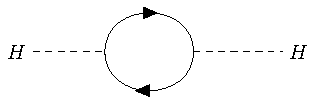
\includegraphics{Images/higgscorrections.pdf}}
Doing the calculations, we see that this diagram is quadratically divergent and it goes like $\Lambda^2y_\Psi^2/16\pi^2$. If we assume that $\Lambda$ is of order of the Planck scale, the suppression coming from the Yukawa coupling is small\marginnote{(Not so) technical term: \textit{this suppression is peanuts}} so if we set $\mu$ to be of order 246 GeV at tree-level, at one-loop it will become of order Planck. There is no hope to get a light Higgs.\\
This problem requires a precise cancellation between the radiative corrections and the tree-level term.\\
The $\nu_R$ is a fermionic field with chiral invariance associated broken by the mass term proportional to the one-loop corrections, so if the mass is light the corrections will be small. This is called \textbf{technical naturalness}. There is no danger in saying that this mass is much smaller than the cut-off scale so it will remain small even after radiative corrections are turned on. If this mass is heavy then we will have the seesaw mechanism: there is a heavy state that integrated out gives us very light state, because the mass of $\nu_L$ is suppressed. This is why it is called seesaw. However, we can also say that the mass is small, much smaller than the Planck scale, in which case this $\nu_R$ is an addition to the SM, it is not heavy new physics but rather light new physics.
\end{kaobox}
\subsection{Lepton Number}
We said there is an accidental U$(1)_{\text{B}}$ symmetry under which leptons do not transform. Is there an accidental symmetry regarding the lepton sector? Without $\nu_R$, the Yukawa term regarding leptons has the following form:
\[
\overline{l}_L^iY_l^{ij}He_R^j
\]
We can transform the doublet and the singlet with two unitary transformations and diagonalize $Y$ without touching the kinetic terms. Without inserting the additional structure for the mass of the neutrinos we do not have any counterpart of the CKM matrix, at this level there is no flavour mixing. We can then go to a basis in which $Y$ is diagonal and at this point then we can change the phases of the three different families independently. There is not one \textbf{lepton number} but there are three: $L_e, L_\mu$ and $L_\tau$. Under $L_e$, both the electron and the electronic neutrino transform with the same charge which is equal to 1 and the others do not transform. Under $L_\mu$ only the muon and the muonic neutrino transform with the same charge while the others do not transform and the same applies for $L_\tau$. It is possible to transform the fermion fields with different phases and this will keep every single term in the Lagrangian invariant. This accidental symmetry is a product of U$(1)_{\text{B}}$ and [U$(1)]^3$.\\
At least at the classical level, these are the exact global symmetries which emerge. Why are they called \textit{accidental}? Because they come as an accident at low energy, in the sense that the UV physics might not have them. In fact, if we write higher dimensional terms, e.g. $O_{\text{Weinberg}}$, we notice that they violate lepton number. If we say that the new physics has this symmetry then such a term is not allowed. But we are not imposing this symmetry by hand, we are just looking at low-energy and see which symmetries come out. This is the power of accidental symmetries: even if the UV theory is not invariant under that symmetry, at low-energy it emerges as an accident, it comes for free. They emerge because the theory is an EFT and because there is a large gap between the scale at which we do the experiments and the UV scale, which is much higher. Higher dimensional operators contribute to the experiments with the inverse power of the cut-off scale, they all violate these symmetries but their effects will be largely suppressed.\\
These symmetries are not truly \textit{exact} symmetries, they are exact only at $D=4$ but if we consider the theory as a whole they are \textit{approximate}. Accidental symmetries are important because they might be the only global symmetries that are allowed in nature because of gravity. This is an important issue when we try to include dark matter in our theory because as far as we can tell is not coming from the SM so we have the extend the theory. Where does the stability of DM come from? People would say \textit{okay, we introduce a global symmetry and make it stable}. Well, there is a problem. One possible way of arguing is that if such global symmetry exist, it is accidental.
\section{Fujikawa Approach to Anomalies}\marginnote{From \cite{We2}, Section 22.2 and 22.4.}
A more direct connection between the anomaly and the violation of a symmetry uses the \textbf{path integral}. The idea, due to Fujikawa, is that anomalies arise when there are symmetries of the action that are not symmetries of the functional measure in the path integral. 
\[
I=\int\pazocal{D}\phi e^{iS[\phi]} 
\]
% \[
% Z[J]=\int\pazocal{D}\phi\exp{iS[\phi]+i\int d^4xJ(x)\phi(x)} 
% \]
If the symmetry is anomalous, then the measure $\pazocal{D}\phi$ is not invariant.\\
Take now a massless fermionic field $\Psi(x)$ interacting electromagnetically with $A_\mu(x)$ as:
\[
\pazocal{L}=-\frac{1}{4}F_{\mu\nu}F^{\mu\nu}+\overline{\Psi}i\gamma^\mu D_\mu\Psi \qquad \left\{
\begin{aligned}
&F_{\mu\nu}=\partial_\mu A_\nu-\partial_\nu A_\mu\\
&\overline{\Psi}=\Psi^\dagger\gamma^0\\
&D_\mu=\partial_\mu-iet^aA_\mu^a
\end{aligned}
\right.
\]
Consider the case in which $\Psi(x)$ transforms as follows:
\[
\Psi(x)\to \Psi'(x)=e^{i\alpha(x)}\Psi(x)
\]
Under such transformation, the action $S=\int d^4x\pazocal{L}$ is invariant for constant $\alpha(x)$. For a local transformation instead we have:
\[
\delta S=\int d^4xJ^{\mu}(x)\partial_\mu\alpha(x) \quad \text{with}\;J^{\mu}=\overline{\Psi}\gamma^\mu\Psi
\]
The path integral measure now has the transformation property:
\[
\pazocal{D}\Psi\pazocal{D}\overline{\Psi}\to\exp{i\int d^4x\alpha(x)\pazocal{A}(x)}\pazocal{D}\Psi\pazocal{D}\overline{\Psi}
\]
where $\pazocal{A}(x)$ is the \textbf{anomaly function}. The measure $\pazocal{D}\Psi\pazocal{D}\overline{\Psi}$ appears in the path integral weighted with a factor $\exp{i\int d^4x\pazocal{L}}$ so the factor which appears in the transformation rule for the integral measure has the same effect as if the Lagrangian was not invariant under such transformation:
\[
\pazocal{L}\to\pazocal{L}+\alpha(x)\pazocal{A}(x)
\]
After calculations that we do not perform, one obtains for the anomaly function:
\[
\pazocal{A}(x)=-\frac{1}{16\pi^2}\epsilon_{\mu\nu\rho\sigma}F^{\mu\nu}_aF^{\rho\sigma}_bD^{abc} \qquad \text{with}\;D^{abc}=\frac{1}{2}\Tr{t^a\{t^b,t^c\}}
\]
% \[
% \pazocal{A}^a(x)=\frac{1}{16\pi^2}D^{abc}F_{\mu\nu}^b\Tilde{F}^{\mu\nu,c} \quad \left\{\begin{aligned}
% &D^{abc}=\frac{1}{2}\Tr{T^a\{T^b,T^c\}}\\
% &\Tilde{F}^{\mu\nu,c}=\frac{1}{2}\epsilon^{\mu\nu\rho\sigma}F_{\rho\sigma}^a
% \end{aligned}\right.
% \]
The change in the path integral over the fermionic fields then become:
\[
i\int d^4x\pazocal{D}\Psi\pazocal{D}\overline{\Psi}e^{iS}[\partial_\mu J^{\mu}(x)\alpha(x)+\alpha(x)\pazocal{A}(x)]
\]
This is just a change of variables so the path integral cannot be affected, so it has to be:\marginnote{
To get this result, keep in mind that it is possible to write: 
\[
J^\mu\partial_\mu\alpha(x)=\partial_\mu(J^\mu\alpha(x))-\alpha(x)\partial_\mu J^\mu
\]
The total derivative term vanishes when integrating in $d^4x$ and the common factor $\alpha(x)$ can be simplified between the $\partial_\mu J^\mu$ term and the $\pazocal{A}(x)$ term.
}
\[
\int\pazocal{D}\Psi\pazocal{D}\overline{\Psi}e^{iS}\partial_\mu J^{\mu}=\pazocal{A}(x)\int\pazocal{D}\Psi\pazocal{D}\overline{\Psi}e^{iS}
\]
To simplify the notation, for a generic operator $O$ it is possible to define its quantum average in a fixed background field $A^\mu(x)$ as:
\[
\Braket{O}_{A_\mu}:=\frac{\int\pazocal{D}\Psi\pazocal{D}\overline{\Psi}O(x)e^{iS}}{\int \pazocal{D}\Psi\pazocal{D}\overline{\Psi}e^{iS}}
\]
and the previous identity becomes:
\[
\Braket{\partial_\mu J^\mu}_{A_\mu}=\pazocal{A}(x)=-\frac{1}{16\pi^2}\epsilon_{\mu\nu\rho\sigma}F^{\mu\nu}_aF^{\rho\sigma}_bD^{abc}
\]
The anomaly function vanishes when $D^{abc}=0$. This happens when:
\begin{itemize}
    \item fields are in vector-like representations of the entire symmetry group, i.e. $\Psi_L$ in a certain representation $r$ and $\Psi_R$ in the same $r$.
    \[
    \Psi_R\to U\Psi_R\Rightarrow\Psi_R^C=U^*\Psi_R^C \quad U=\exp{i\alpha^aT^a}
    \]
    The generators can be written as $T^a=\text{diag}(t_L^a, -t_R^{aT})$ but in a vector-like representation we know that $t_L=t_R$:
    \begin{align*}
    D^{abc}&=\frac{1}{2}\Tr{T^a\{T^b,T^c\}}=\frac{1}{2}\Tr{t_L^a\{t_L^b,t_L^c\}}-\frac{1}{2}\Tr{(t_R^a)^T\{(t_R^b)^T,(t_R^c)^T\}}\\
    &=\frac{1}{2}\Tr{t_L^a\{t_L^b,t_L^c\}}-\frac{1}{2}\Tr{t_R^a\{t_R^b,t_R^c\}}=0
    \end{align*}
    This tells us that QCD is anomaly free, [SU$(3)_{\text{C}}]^3=0$ because it is vector-like.
    \item fields are in (pseudo-) real representations.\\
    This means that given a matrix $U$ such that $U^*=SUS^{-1}$, the representation $r$ is pseudo-real if it transforms under $U$. Moreover, if $T^a$ are purely imaginary then the representation $r$ is real. We know that the fundamental of SU(2) is a real representation:
    \[
    (T^a)^T=-ST^aS^{-1}
    \]
    It then follows that:
    \begin{align*}
    D^{abc}&=\frac{1}{2}\Tr{T^a\{T^b,T^c\}}=\frac{1}{2}\Tr{(T^a)^T\{(T^b)^T,(T^c)^T\}}(-1)^3\\
    &=-D^{abc}\Rightarrow D^{abc}=0
    \end{align*}
\end{itemize}
Groups with only real or pseudo-real representations are SO$(2n+1)$, SO$(4n)$ for $n\ge2$ and Sp$(2n)$ for $n\ge3$. Moreover, groups with complex representations but vanishing anomalies are SO$(4n+2)$ except for SO(2)=U(1) and SO(6)=SU(4). Anomalies are then possible only for algebras that include SU$(n)$ (for $n\ge3$) or U$(1)$ factors. As we know, this is the case of the Standard Model, so we must rely on cancellation among quarks and leptons to make the group anomaly free.\\
Given this discussion about anomalies, we ask ourselves: \textit{is baryon number a good symmetry? Does it have any anomaly?}\\
% \[
% \left\{
% \begin{aligned}
% &q_L=\Box_{1/3}\,\text{of SU$(3)_{\text{C}}\times$U$(1)_{\text{B}}$} &&q_L=\begin{pmatrix}u_L\\d_L\end{pmatrix}\to q_L=\overbrace{(\Box,1/3)}^{r}\\
% &q_R=\Box_{1/3}\,\text{of SU$(3)_{\text{C}}\times$U$(1)_{\text{B}}$} &&q_R=(u_R,d_R)\to q_R^c=\overbrace{(\overline{\Box},1/3)}^{\overline{r}}
% \end{aligned}
% \right.
% \]
There is no anomaly of baryon number under SU$(3)_{\text{C}}$ because they transform under a real representation. Under SU$(2)_{\text{EW}}$ we have:
\[
D^{Bbc}=\frac{1}{2}\Tr{B}_{\text{weak doublets}}\Tr{\{T^b,T^c\}}=\frac{1}{2}\underset{\mathclap{\tikz \node {$\uparrow$} node [below=1ex] {\footnotesize  charge};}}{\frac{1}{3}}\cdot\overset{\mathclap{\tikz \node {$\downarrow$} node [above=1ex] {\footnotesize  colour};}}{3}N_f\delta^{bc}=N_f\frac{\delta^{bc}}{2}\marginnote{In the weak doublets, only $q_L$ contributes and it is factored out because it acts on a different space.}
\]
With the same strategy, we can compute the anomaly content under U$(1)_{\text{Y}}$:
\begin{align*}
D^{Byy}&=\frac{1}{2}\Tr{B}_{\text{quarks}}\Tr{\{Y,Y\}}\xleftarrow[]{}\;=2Y^2\\
&=3N_f\left[\frac{1}{3}\cdot2\cdot\left(-\frac{1}{6}\right)^2+\left(-\frac{1}{3}\right)\cdot\left(-\frac{2}{3}\right)^2+\left(-\frac{1}{3}\right)\cdot\left(\frac{1}{3}\right)^2\right]\\
&=N_f\left[\frac{1}{18}-\frac{4}{9}-\frac{1}{9}\right]=-\frac{N_f}{2}
\end{align*}
This results in:
\[
\Braket{\partial_\mu J^\mu_B}=\frac{1}{16\pi^2}\frac{N_f}{2}[W_{\mu\nu}^i\Tilde{W}^{\mu\nu,i}-B_{\mu\nu}\Tilde{B}^{\mu\nu}]
\]
which is not a symmetry. At the classical level, there is a symmetry given by the product of baryon number and the three lepton numbers while at the quantum level instead we have:
\[
\text{U}(1)_{\text{B$-$L}}\times\text{U}(1)_{L_e-L_\mu}\times\text{U}(1)_{L_e-L_\tau}
\]
which is an accidental symmetry of the SM. In particular, B$-$L is anomalous and this is important if we want to extend the SM because it is not possible to gauge it.
% Suppose now that B$-$L is promoted to a gauge symmetry, what we need to check is [U$(1)_{\text{B$-$L}}]^3$ which is different from 0 in the SM but equal to 0 when we add $\nu_R$.
\section{SU(5) Grand Unification Theory}\marginnote[-1cm]{From \cite{CL}, Chapter 14.}
Elementary particle interactions are correctly described by the gauge group SU$(3)\times$SU$(2)\times$U$(1)$ down to distances as small as $10^{-16}$\,cm: QCD is the strong interaction theory and the Glashow-Weinberg-Salam model provides the theory of weak and electromagnetic interaction. It is desirable to have a more unified theory which can combine all three of these interactions as components of a single force, a theory with only one gauge coupling.\\
Georgi and Glashow showed that for the Standard Model the simplest unification gauge group of colour and flavour is SU(5) but because of the large differences in coupling strengths of strong and electroweak interactions, this unification would not become apparent until the energy scale of $10^{14}$ \,GeV, i.e. a distance of $10^{-28}$\,cm.\\
A general representation under an SU(5) transformation may be expressed as:
\[
\Psi^{ij\cdots}_{kl\cdots}\to U^i_mU^j_nU^s_kU^t_l\cdots\Psi^{mn\cdots}_{st\cdots}
\]
where all the indices run from 1 to 5 and:
\[
U^i_m=\exp{i\alpha^a\frac{\lambda^a}{2}}^i_m
\]
is a $5\times5$ unitary matrix. $\lambda^a$ with $a=0,1,\cdots,23$ is a set of 24 $5\times5$ generalized Gell-Mann matrices which are hermitian and traceless with normalization given by $\Tr{\lambda^a,\lambda^b}=2\delta^{ab}$. To obtain the SU$(3)\times$SU$(2)$ content of a representation we identify the first three of the SU(5) indices as the colour indices and the remaining two as SU$(2)_{\text{L}}$ indices:
\[
i=(\alpha,r) \quad \alpha=1,2,3 \quad r=4,5
\]
One family of fermions can be accommodated in an SU(5) reducible representation of $\overline{5}+10$:
\[
\overline{5}:\left(\begin{array}{c}
d_1^c\\d_2^c\\d_3^c\\l=\begin{pmatrix}\nu\\e
\end{pmatrix}
\end{array}\right) \quad
10: \left(\begin{array}{ccc:cc}
0 & u_3^c & -u_2^c & u_1 & d_1\\
-u_3^c & 0 & u_1^c & u_2 & d_2\\
u_2^c & -u_1^c & 0 & u_3 & d_3\\
\hdashline
-u_1 & -u_2 & -u_3 & 0 & e^+\\
-d_1 & -d_2 & -d_3 & -e^+ & 0
\end{array}\right)
\]
One consequence of the SU(5) scheme is an explanation for the experimentally observed charge quantization. This is because the eigenvalues of the generators of a simple non-abelian group are discrete while those corresponding to the abelian U(1) group are continuous.\marginnote{e.g. in the SO(3) group of rotations, the eigenvalues of the third component of the angular momentum can take only integer or half-integer values while in the U(1) symmetry of translation invariance in time there is no restriction on the eigenvalues of the corresponding generators.} Therefore in the SU(5) theory, since the electric charge $Q$ is one of the generators, its eigenvalues are discrete and hence quantized. The electric charge is an additive quantum number, so $Q$ must be some linear combination of the diagonal generators in SU(5). We then have:
\[
Q=T_3+\frac{1}{2}Y=T_3+cT_0
\]
where $T_3$ and $T_0$ are the diagonal generators belonging to the SU(2) and U(1) subgroups respectively.
\[
T_3=\frac{\lambda_3}{2}=\mqty(\dmat{0,0,0,\frac{1}{2},-\frac{1}{2}}) \quad T_0=\frac{\lambda_0}{2}=\frac{1}{\sqrt{15}}\mqty(\dmat{1,1,1,-\frac{3}{2},-\frac{3}{2}})
\]
The coefficient $c$ can be obtained by comparing the values of $T_0$ provided above and the hypercharge of the particles in the $\overline{5}$, giving us:
\[
c=-\sqrt{\frac{5}{3}}
\]
To check this result, we note that for the fundamental representation, combining all our knowledge discussed here we get:
\[
Q=\mqty(\dmat{-\frac{1}{3},-\frac{1}{3},-\frac{1}{3},1,0}):=Q_i\delta_{ij}
\]
and it follows that the fundamental conjugate representation $\overline{5}$ has $Q=-Q_i\delta-{ij}$. The most interesting aspect of charge quantization is the relation between colour SU(3) and charge. The traceless condition for the charge operator requires, for three colours:
\[
3Q_d+Q_{e^+}=0
\]
Quarks carry one third of the lepton charge because they have three colours. SU(5) then provides a rational basis for understanding particle charges.\\
The SU(5) adjoint representation has dimension $5^2-1=24$ and the following SU$(3)\times$SU$(2)$ decomposition:
\[
24=(8,1)+(1,3)+(1,1)+(3,2)+(\overline{3},2)
\]
$A_\beta^\alpha$ (8,1) are the SU(3) gluons $G_\beta^\alpha$, $A_s^r$ (1,3) are the three SU(2) vector fields $W$ and (1,1), given by a linear combination of $A_\alpha^\alpha$ and $A_r^r$ is the U(1) $B$-field. The remaining 12 fields have both SU(3) and SU(2) indices and they are denoted as $X,Y$ gauge bosons. These vector particles carry fractional charge:
\[
Q_X=-\frac{4}{3} \quad Q_Y=-\frac{1}{3}
\]
All the SU(5) gauge bosons can be put in a $5\times5$ matrix $A$ of the form:
\[
A=\frac{1}{2}\sum_{a=0}^{23}A^a\lambda^a
\]
\subsection{Proton Decay}
One prominent feature of the Grand Unification Theory is the non conservation of the baryon number. In the SM, baryon and lepton number are accidental, while the combination $B+L$ is anomalous: there is no proton decay mediated by anomalies.  The SU(5) model has this property and the leading effective Lagrangian for proton decay arises from a set of tree-level $X$ boson exchange diagrams. $X$ bosons couple to two-fermion channels with different baryon numbers:\\
\begin{figure}[h]
    \centering
    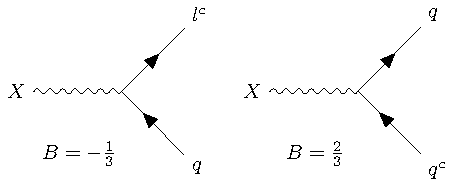
\includegraphics[width=0.7\textwidth]{Images/baryonnumber.pdf}
    \caption*{}
    \labfig{bnumber}
\end{figure}\\
In the case on the left, they couple to quarks and leptons so they are referred as \textbf{leptoquarks} while in the case on the right they transform quarks to antiquarks and they are called \textbf{diquarks}.\\
Consequently, through the mediation of a $X$ boson a $B=-1/3$ channel can be converted into a $B=2/3$ one, i.e. a baryon number changing process $(\Delta B=1)$ occurs at tree-level.\\
\begin{figure}[h]
    \centering
    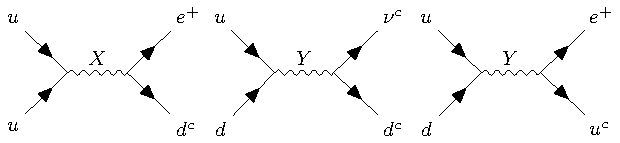
\includegraphics{Images/xyy.pdf}
    \caption*{}
    \labfig{xyy}
\end{figure}\\
$B-L$ is conserved, so a process like $p\to\pi^0e^+$ is allowed but not $n\to\pi^+e^-$. $B+L$ is instead violated, what are the operators accounting for such violation? These are dimension 6 $(B+L)$-violating operators:
\[
\frac{g^2_{\text{GUT}}}{M^2_{\text{GUT}}}u^{c\dagger}qe^{c\dagger}q \quad \frac{g^2_{\text{GUT}}}{M^2_{\text{GUT}}}u^{c\dagger}qd^{c\dagger}l 
\]
At Super-Kamiokande they measured $\tau(p\to\pi^0e^+)\ge1.4\cdot10^{34}$\,years resulting in $M_{\text{GUT}}\gtrsim10^{16}$\,GeV\marginnote[-2cm]{I am 0\% sure of what is written here because my notes on this part are terrible and there was someone using a drill in this exact moment so even the recording of the lecture is useless.}
\section{Custodial Symmetry}
\textbf{Custodial symmetry} is defined as a symmetry which remains after spontaneous symmetry breaking and that can prevent higher-order radiative corrections from spoiling some property of the theory.\\
In the SM, this is a residue global SU(2) symmetry of the Higgs potential:
\[
V(H)=-\mu^2H^\dagger H+\lambda(H^\dagger H)^2 \quad H=\begin{pmatrix}\phi_1+i\phi_2\\\phi_3+i\phi_4\end{pmatrix}
\]
The potential is invariant under SO(4), with a transformation of the form:
\[
\phi_i\to\phi_i'=R_{ij}\phi_j \quad RR^T=\mathbb{1}
\]
When $H$ acquires a vev, SO(4) is spontaneously broken to SO(3):
\[
\Braket{H}=\begin{pmatrix}0\\\frac{v}{\sqrt{2}}\end{pmatrix}\xleftrightarrow[]{}\Braket{\Phi}=\begin{pmatrix}0\\0\\\frac{v}{\sqrt{2}}\\0\end{pmatrix} \;\text{where}\;\Phi=\begin{pmatrix}\phi_1\\\phi_2\\\phi_3\\\phi_4\end{pmatrix}
\]
There exists an unbroken SO(3) that acts on entries 1,2 and 4 of $\Phi$. Remember that for SO$(n)$ there are $n(n-1)/2$ generators:
\[
\begin{cases}
n=4 \;\text{has 6 generators}\\
n=3 \;\text{has 3 generators}
\end{cases}
\Rightarrow 3\,\text{NGB}
\]
Looking at the algebras, we know that $\mathfrak{so}(3)\sim\mathfrak{su}(2)$ while the relation for SO(4) is given by $\mathfrak{so}(4)\sim\mathfrak{su}(2)\times\mathfrak{su}(2)$.
\begin{kaobox}[frametitle=More on SO(4) algebra]
It is also possible to write an exact relation of the previous one:
\[
\text{SO}(4)=\frac{\text{SU}(2)_{\text{L}}\times\text{SU}(2)_{\text{R}}}{\mathbb{Z}_2}
\]
Take now a vector of $\mathbb{R}^4$ denoted by $v^a$ which transforms under SO(4) as:
\[
v^a\to v'^a=R^{ab}v^b \quad a,b=1,2,3,4
\]
From this vector we can define $V:=v^aT^a$ where $T^a=\{i\Vec{\sigma},\mathbb{1}\}$ and $V$ is a $2\times2$ matrix. The transformation rule under SU$(2)_{\text{L}}\times$SU$(2)_{\text{R}}$ is the following:
\[
V\to V'=LVR^\dagger \quad L\in\text{SU}(2)_{\text{L}}, R\in\text{SU}(2)_{\text{R}}
\]
What is the connection with SO(4)? Compute the determinant of $V$:
\[
\det V=\det\left(\begin{array}{cc}
    v_4+iv_3 & iv_1+v_2 \\
    iv_1-v_2 & v_4-iv_3
\end{array}\right)=\sum_{i=1}^4(v_i)^2=\norm{\Vec{v}}^2
\]
When transforming $V$ under SU$(2)_{\text{L}}\times$SU$(2)_{\text{R}}$, the determinant remains the same therefore we have that $\norm{\Vec{v}}=\norm{\Vec{v}'}$. We can also define $v^a$ as:
\[
v^a:=\frac{1}{2}\Tr{T^{a\dagger}V}=\frac{1}{2}v^b\Tr{T^{a\dagger}T^b}=\frac{1}{2}v^b\delta^{ab}
\]
which transforms as:
\[
v'^a=\Tr{T^{a\dagger}V'}=\underbrace{\Tr{T^{a\dagger}LT^bR^\dagger}}_{:=R^{ab}}v^b
\]
\end{kaobox}
The point is that for each element of SO(4) we have two elements of SU$(2)_{\text{L}}\times$SU$(2)_{\text{R}}$. SO(4) broken to SO(3) is the same as SU$(2)_{\text{L}}\times$SU$(2)_{\text{R}}$ broken to SU$(2)_{\text{V}}$ but this is something familiar: it is the chiral symmetry breaking in QCD with 2 flavours.\\
In the SM the masses of the $W$ and the $Z$ bosons are known and given by:%\marginnote{From \cite{schwartz}, Section 31.2.}
\[
m_W^2=\frac{v^2}{4}g^2 \quad m_Z^2=\frac{v^2}{4}(g^2+g'^2)
\]
It turns out that $m_Z=m_W$ if $g'=0$ but it is not the case. However, their ratio is determined by the relative strengths of the weak and electromagnetic gauge couplings:
\[
\frac{m_W^2}{m_Z^2}=\frac{g^2}{g^2+g'^2}=\cos^2\theta_w
\]
This is a consequence of the way the SU$(2)\times$U(1) symmetry is spontaneously broken through the Higgs mechanism with a single SU(2) doublet. If the Higgs sector was more complicated, there might be deviations from this even at tree-level. It is therefore useful to define the $\rho$-parameter:
\[
\rho:=\frac{m_W}{m_Z\cos\theta_w}
\]
Denoting the tree-level value of $\rho$ as $\rho_0$ we see that $\rho_0=1$ in the Standard Model. What exactly guarantees that $\rho_0=1$? This is guaranteed by the symmetry we just discussed: the Higgs potential is invariant under SO(4), which has 6 generators, and when $H$ gets a vev the SO(4) symmetry is broken to SO(3). There is a residual global SU(2) symmetry after electroweak symmetry breaking which is known as \textbf{custodial isospin}, or \textbf{custodial SU(2)}.\\
In order to see corrections to the $\rho$-parameter, we can exploit the similarity with the Sigma model and rewrite the Higgs sector in terms of a new field $\pazocal{H}$:
\[
\pazocal{H}:=\frac{v+h(x)}{\sqrt{2}}\Sigma(x) \quad \Sigma(x)=\exp{i\frac{\chi^a\sigma^a}{v}}
\]
This is nothing but the product of the doublet $H$ and $H^c$ both seen as columns, i.e. $\pazocal{H}=[(H)(H^c)]$. In fact, it is possible to see that:
\[
\pazocal{H}^\dagger\pazocal{H}=\left(\begin{array}{cc}
    H^\dagger H & H^\dagger H^c \\
    H^{c\dagger}H & H^{c\dagger}H^c
\end{array}\right)=H^\dagger H\cdot\mathbb{1}\marginnote{This is because $H^{c\dagger}H^c=H^\dagger H$ and $H^{c\dagger}H=H^\dagger H^c=0$. Contino did not give much explanations about this, just \textit{convince yourself it is true} and \textit{prove it}.} 
\]
The potential can be now written in terms of $\pazocal{H}$ as follows:
\[
V(H)=-\frac{\mu^2}{2}\Tr{\pazocal{H^\dagger\pazocal{H}}}+\frac{\lambda}{4}\left(\Tr{\pazocal{H}^\dagger\pazocal{H}}\right)^2=-\frac{\mu^2}{2}(v+h)^2+\frac{\lambda}{4}(v+h)^4
\]
For the kinetic term instead we write:
\begin{align*}
\partial_\mu H^\dagger\partial^\mu H&=\frac{1}{2}\Tr{(\partial_\mu\pazocal{H}^\dagger)(\partial^\mu\pazocal{H}^\dagger)}\\
&=\frac{1}{2}(\partial_\mu h)^2+\frac{(v+h)^2}{4}\Tr{(\partial_\mu\Sigma^\dagger)(\partial^\mu\Sigma)}
\end{align*}
It turns out that it is possible to covariantize it and what we obtain is:
\[
D_\mu H^\dagger D^\mu H=\frac{1}{2}(\partial_\mu h)^2+\frac{(v+h)^2}{4}\Tr{(D_\mu\Sigma^\dagger)(D^\mu\Sigma)}
\]
where the covariant derivative is defined as:
\[
D_\mu\Sigma=\partial_\mu\Sigma-igW_\mu^a\frac{\sigma^a}{2}\Sigma+ig'\Sigma YB_\mu
\]
What is left to write is the Yukawa term, e.g. for quarks:\marginnote{For leptons is the same thing.}
\[
\pazocal{L}_{\text{Yuk}}\supset-\overline{q}_L^iY_u^{ij}H^cu_R^j-\overline{q}_L^iY_d^{ij}Hd_r^j+\text{h.c.}=-\overline{q}_L^i\pazocal{H}\left(\begin{array}{cc}
    Y_u^{ij} & u_R^j \\
    Y_d^{ij} & d_R^j
\end{array}\right)+\text{h.c.}
\]
The fact that $m_u-m_d\neq0$ is another explicit breaking of SU$(2)_{\text{R}}$, hence of the custodial of SO(3). In particular, the most important effects come from top and bottom so we can consider the corrections at one-loop to the $W$ and $Z$ bosons coming from the virtual exchange of the top and bottom.
\begin{figure}[h]
    \centering
    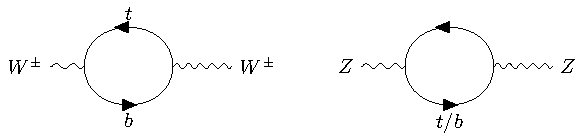
\includegraphics{Images/wztb.pdf}
    \caption*{}
    \labfig{wztb}
\end{figure}\\
If the masses of the top and the bottom were the same, these contributions would be the same but since the masses are different we have different corrections, $\delta m_Z\neq\delta m_W$. This implies $\Delta\rho\neq0$, in particular $\rho=1+\Delta\rho$. We can actually forget about the bottom, it is the top contribution which is relevant. $\Delta\rho\approx1/200$ which is in very good agreement with data, in fact experimentally we have $|\rho-1-\Delta\rho^{\text{SM}}|\lesssim10^{-3}$. This means that if we want to extend the SM we better not screw up with custodial symmetry because if we construct a new physics theory which violates at order one the custodial symmetry then that is ruled out. The custodial symmetry violation should be small, this is the message from data.
\section{Non-Linear EW Lagrangian}
Since the custodial symmetry is an accidental symmetry, there should be some higher dimensional operators which accounts for its breaking. Which operator is breaking the symmetry? If we focus on the Higgs sector there is only one operator of dimension 6, given by $(H^\dagger\overset{\leftrightarrow}{D_\mu}H)^2$. In the unitary gauge, this would give a contribution to the mass of the $Z$ boson because the covariant derivative is sandwiched between two $H$ and we would get only the neutral component not the charged one. This means that custodial symmetry is violated.\\
There is another way to see that this operator breaks custodial symmetry. The theory can be reformulated in the following way:
\begin{align*}
\pazocal{L}=&\pazocal{L}_{\text{kin}}(\Psi)+\pazocal{L}_{\text{kin}}(\text{gauge})+\frac{1}{2}(\partial_\mu h)^2+\frac{(v+h)^2}{4}\Tr{(D_\mu\Sigma^\dagger)(D^\mu\Sigma)}\\
&-\overline{q}_L^i\Sigma\left(\begin{array}{cc}
    Y_u^{ij} & u_R^j \\
    Y_d^{ij} & d_R^j
\end{array}\right)\frac{(v+h)}{\sqrt{2}}+\text{h.c.}-V(h)
\end{align*}
Notice that $h(x)$ is a singlet of SO(4) so there is no covariant derivative here but we can think of $h$ as sort of the norm of $H^\dagger H$, which is an invariant of SU$(2)\times$U(1). We already saw a theory of this kind when we discussed the SU$(2)\times$SU(2) breaking in the previous course\marginnote{See \cite{EW}, Section 3.10 for more details about SU$(2)\times$SU(2) breaking.}.
\begin{kaobox}[frametitle=Remark on SU(2)$\times$SU(2) symmetry breaking]
If we put only the three NGBs coming from the breaking then the scattering amplitudes at high energies grow and the theory becomes non perturbative. We then had to introduce an additional degree of freedom, the Higgs boson $h$, in such a way that the scattering amplitude coming from $\chi\chi\to\chi\chi$ would be exactly canceled by the Higgs contribution. This is because we introduced $h$ in this way and the way to see that this cancellation must occur is that we can rewrite this in terms of a renormalizable Lagrangian where there are no dimensionful couplings so there should be no dependency on the energy except for the usual running of the couplings.\\
We did this thinking for example in terms of QCD. In QCD there are these three pions and we can try to do the same: is it possible to make things well behaved at high energies? We introduce an extra degree of freedom and make a linear sigma model instead of a non-linear one. There is such a particle with the quantum numbers of the radial mode, which is the sigma particle, but this sigma particle does not couple in this way. First of all, it has a very large mass and second of all the mass is even complicated to define.\\ 
% If we do an experiment and see the resonance then it is really broad, that's why it is useful to define a mass, which means that eventually we will not have small couplings.\\
\end{kaobox}
At the level of the global symmetry breaking there is the same pattern both in QCD and in the electroweak sector but the latter is including one degree of freedom which completes the theory into something renormalizable, while in the case of QCD this is not true. In QCD the theory becomes strongly coupled as we increase the energy while if we do the same scattering with $\chi$ the amplitude grows but at a certain point it is saturated because there is the Higgs boson which switches on and the theory stays weakly coupled. Experimentally, how precisely do we know the Higgs coupling? It seems that having couplings exactly equal to those of this Lagrangian is crucial because otherwise the cancellation does not occur anymore. So the question is: \textit{does the Standard Model reproduce nature or not?} The couplings could be equal to the SM values plus small corrections. How can we write a theory where the Higgs boson has a different coupling? We can simply relax some of our assumptions, here the assumption is that the SU$(2)_{\text{EW}}\times$U$(1)_{\text{Y}}$ symmetry is realized linearly at high energies, at $E\gg v$ we can forget about the breaking and the symmetry is realized linearly so all the fields have to come in multiplets of this symmetry. We could in principle relax this so what we need to account for is the fact that the $W$ and the $Z$ bosons are massive, that's the experimental evidence. Of course we need to have this symmetry which has to be spontaneously broken, there should be the Higgs mechanism, everything is the same but we do not need to ask for a linear realization at high energies. We could completely eliminate the Higgs boson from the theory, and that's basically what we have in technicolor theories, or we can introduce it but without requiring that the symmetry is realized linearly. This means that we need to construct a Lagrangian which has the global symmetry SU$(2)\times$SU(2) broken to SU(2) and then we gauge the subgroup, we do not impose that it has to reconstruct linear multiplets. Considering all terms which are invariant under the symmetry, the most general Lagrangian we can write is:
\begin{align*}
\pazocal{L}=&\pazocal{L}_{\text{kin}}(\Psi)+\pazocal{L}_{\text{kin}}(\text{gauge})+\frac{1}{2}(\partial_\mu h)^2\\
&-\frac{v}{\sqrt{2}}\overline{q}_L^i\Sigma\left(\begin{array}{cc}
    Y_u^{ij} & u_R^j \\
    Y_d^{ij} & d_R^j
\end{array}\right)\left(1+c_q\frac{h}{v}+\cdots\right)\\
&+\frac{v^2}{4}\Tr{(D_\mu\Sigma^\dagger)(D^\mu\Sigma)}\underbrace{\left(1+2c_v\frac{h}{v}+c_{2v}\frac{h^2}{v^2}+\cdots\right)}_{\text{singlet of SU$(2)\times$SU(2)}}-V(h)
\end{align*}
where the potential is given by:
\[
V(h)=-\frac{m_h^2}{2}h^2(x)+c_3\frac{m_h^2}{6v}h^3(x)+c_4\frac{m_h^2}{v^2}h^4(x)+\cdots\marginnote{Maybe in literature $c_3$ and $c_4$ are called $\lambda_3$ and $\lambda_4$.}
\]
In the SM limit, $c_v=1$ and $c_{2v}=1$. In other words, these two parametrize the following interactions:
\begin{figure}[h]
    \centering
    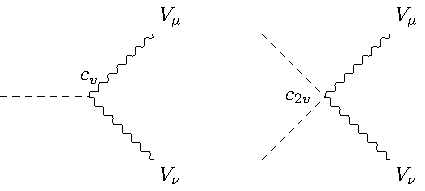
\includegraphics[width=0.7\textwidth]{Images/cvc2v.pdf}
    \caption*{}
    \labfig{cvc2v}
\end{figure}\\
This Lagrangian makes sense because it is invariant under SU$(2)\times$U(1), of course only for these values we can reconstruct the Higgs boson but for values of these parameters different from 1 we still have gauge invariance but the symmetry is not realized linearly not because of a lack of degrees of freedom. For the other parameters, the SM is realized for $c_q=1$, $c_3=1$ and $c_4=1$. The theory is not renormalizable so it will blow up at a certain point but who cares, it is an EFT but we knew it from the beginning. Where is the cut-off? Here it has to be, without a doubt, a few TeV because that is the energy at which couplings blow up. This is the \textbf{non-linear electroweak Lagrangian} and it is constructed by making fewer assumptions than the SM, we ask for SU$(2)\times$U(1) symmetry but we do not ask for linearity.\\
Somebody may complain: the kinetic term we wrote for $\Sigma$ is the term which follows if we impose an invariance under SU$(2)\times$SU(2) and then we gauge SU$(2)\times$U(1). However, here the custodial symmetry is not imposed by hand, we do not want to say that it is necessarily recovered if we switch off the gauging. That was true for the linear Lagrangian, because the first operator which breaks custodial symmetry arises at dimension 6 level. In that case, custodial symmetry was accidental at low energy, is it true also here? The answer is no, because if we do not impose that by switching off the gauging we recover custodial symmetry then there is another kinetic term that we can write. Remember that the rule of this game is that we have to have local invariance under SU$(2)\times$U(1) but we are not imposing custodial symmetry. If we do not impose custodial symmetry then there is another term that we can write which is invariant only under SU$(2)\times$U(1). How can we write it? First of all let's recall that $\Sigma$ transforms as $\Sigma\to L\Sigma R^\dagger$ with $L\in\text{SU}(2)_{\text{L}}$, $R\in\text{SU}(2)_{\text{R}}$ and hypercharge is the third generator of SU$(2)_{\text{R}}$. It is then possible to construct the following objects:
\[
\Sigma^\dagger D_\mu\Sigma\to R(\Sigma^\dagger D_\mu\Sigma)R^\dagger \quad \Sigma D_\mu\Sigma^\dagger\to L(\Sigma D_\mu\Sigma^\dagger)L^\dagger
\]
The kinetic term can also be rewritten as:
\[
\Tr{D_\mu\Sigma^\dagger D^\mu\Sigma}=\Tr{\Sigma^\dagger D_\mu\Sigma\sigma_3\Sigma^\dagger D_\mu\Sigma\sigma_3}
\]
It is clear that we have one of these two objects and we are making the square and then we take the trace. Of course we can take either the right-handed or the left-handed term, it is the same. The other kinetic term comes from by noticing that there has to be invariance under SU$(2)_{\text{L}}$ but we do not impose invariance under SU$(2)_{\text{R}}$ and only invariance under U$(1)_{\text{Y}}$ which is inside SU$(2)_{\text{R}}$. We can also write a double trace operator:
\[
\left[\Tr{\Sigma^\dagger D_\mu\Sigma\sigma_3}\right]^2\frac{\alpha_Tv^2}{8}
\]
Without putting the $\sigma_3$ matrix this operator would be 0 because we can easily show that the trace of such quantity is 0. This term is invariant under SU$(2)_{\text{L}}\times$U$(1)_{\text{Y}}$ but not under SU$(2)_{\text{L}}\times$SU$(2)_{\text{R}}$ and it breaks custodial symmetry. If we now go to the unitary gauge where $\Sigma$ is equal to the identity, from the trace of the covariant derivative times $\sigma_3$ we get the mass terms of the $W$ and $Z$ bosons:
\[
m_W^2=\frac{v^2}{4}g^2 \quad m_Z^2=\frac{v^2}{4}(g^2+g'^2)v^2(1+\alpha_T)\Rightarrow\rho=\frac{1}{1+\alpha_T}\neq1
\]
Why such a term was not appearing in the linear realization? Well it is appearing but at dimension 6. The point is that incorporating the fourth degree of freedom into a Higgs doublet forces this effect arising at dimension 6. Custodial symmetry in this formulation does not appear as accidental, this breaking is at the same order of the kinetic term and the parameter $\alpha_T$ has to be very small. The Lagrangian is an effective description of our physics valid up to a certain cut-off scale at which we integrate out the heavy fields. Because this UV dynamics respects the custodial symmetry, this parameter will be small. Then we do experiments at low energy so this parameter $\alpha_T$ would run and we see radiative corrections from UV effects. The point is that if we allow the UV dynamics to be completely general then this $\alpha_T$ would be of order 1 and the $\rho$-parameter would be too large, therefore we have to assume whatever physics we are integrating out has to be custodial invariant to a very good degree, corrections must be very small.\\
% Let's clarify a bit which is the expansion we are assuming. There is a double expansion. First, similarly to the chiral Lagrangian in QCD, there are high order terms which involve a number of derivatives divided by the currents. These terms would give us effects of order energy at which we do experiments divided by $\Lambda$. Notice that here we are not expanding in power of the fields divided by $\Lambda$ because fields might have dimensionality zero. We are expanding in derivatives divided by $\Lambda$ and then of course we are also expanding in the number of Higgs boson fields. This is not really an expansion but it is a way to organize the terms so at a certain Higgs order in the number of $H$ fields we have a finite number of terms but it is clear that the more Higgs fields we have the larger will be the number of Higgs particles involved in our process. E.g. if we have a process with only one Higgs field, then we can stop at the level of one Higgs field in the Lagrangian. This is not true if we have the Higgs doublet, because it acquires a vev so if we have ten of these fields we can still get a contribution zero to a process with zero physical Higgs bosons, simply by putting vev in all these fields. While here we separated the vev from the physical excitation so the more fields $h$ we have the more Higgs particles there will be in our process. Plus we have an expansion in derivatives, this is the double expansion we have.\\
Notice that if we compare with the linear Lagrangian which is a function of $H$ this also has to be thought as an EFT so we have the terms with dimension 4 plus terms with higher dimension. Here indeed we are expanding in numbers of fields because every time we put a field it has dimension 1 so we expand in the number of derivatives and also in the number of fields because they give us the dimensionality. However, the matching is not straightforward because an operator which obtains a certain number of $H$ fields does not correspond to a single operator. For example, this gives a cubic interaction between the Higgs and the vector boson, the interaction vertex is modified by the parameter $c_v$.
\begin{figure}[h]
    \centering
    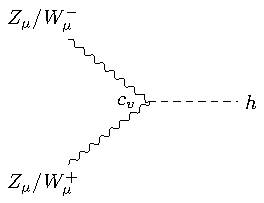
\includegraphics[width=0.45\textwidth]{Images/zwcv.pdf}
    \caption*{}
    \labfig{zwcv}
\end{figure}\\
How can we modify the same interaction in the linear formulation? There will not be any term at dimension 4 because those are the terms of the SM so they have to be terms coming from higher dimension operators. Corrections to this vertex come from dimension 6 operators. In the assumption of only 1 family, at $D=5$ there is only one operator, the Weinberg one, but at $D=6$ there are 59 operators, which are a lot. Some of them were considered even before studying the Higgs physics, e.g. $(H^\dagger D_\mu H)^2$ gives $\Delta\rho$ which has not necessarily anything to do with the Higgs physics. On the other hand, some of them modify \textit{only} the Higgs physics and before the discovery of the Higgs at LHC they were not testable.
\[
O_{WW}=H^\dagger HW_{\mu\nu}^iW^{\mu\nu,i} \quad O_{BB}=H^\dagger HB_{\mu\nu}B^{\mu\nu} \quad O_{GG}=H^\dagger HG_{\mu\nu}^aG^{\mu\nu,a}
\]
If we set $H$ to the vev, they give us some terms which are already present in the Lagrangian. For example, $O_{WW}$ gives the kinetic term of the $W$ in this way. These operator gives cubic interaction but not of the form seen before because they now give vertices with two derivatives.
Then there is another one of the form:
\[
O_H=[\partial_\mu(H^\dagger H)]^2\supset v^2(\partial_\mu h)^2
\]
which vanishes if we set $H$ to the vev and it is only modifying the kinetic term of the Higgs boson. Since it gives a correction to the kinetic term if we renormalize it then this correction will appear in all vertices.
\[
|D_\mu H|^2+c_HO_H\supset\frac{1}{2}\left(1+\frac{c_Hv^2}{2}\right)(\partial_\mu h)^2\marginnote{$c_H$ has dimension $-2$.}
\]
This means that it is possible to redefine $h(x)$ and get:
\[
h(x)\to\frac{h(x)}{\sqrt{1+\frac{c_Hv^2}{2}}}\simeq\left(1-\frac{c_Hv^2}{4}\right)h(x)
\]
The point is that since we want to normalize canonically the kinetic term, then in every vertex where there is a factor $h$ we will get this factor here and this is universal, it is a modification to any coupling in the same way. In particular, $c_v$ will get a contribution from $O_H$:
\[
c_v=1-\frac{c_Hv^2}{4}
\]
At dimension 6 there are other operators which modify the couplings of the fermions, because we can write operators of this form:
\[
O_\Psi=H^\dagger H\overline{\Psi}_LH\Psi_R
\]
where $\Psi$ is either a quark or a lepton. This will give us the correction to the coupling of fermions with the Higgs field.
\begin{figure}[h]
    \centering
    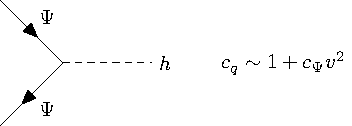
\includegraphics[width=0.6\textwidth]{Images/cq.pdf}
    \caption*{}
    \labfig{cq}
\end{figure}\\
Then there is an operator called $O_6$ of the form:
\[
O_6=(H^\dagger H)^3
\]
which affects the potential, i.e. the Higgs self interaction, in particular it will modify the cubic and quartic interaction and generates higher order interactions involving 5 or 6 Higgs bosons which are really impossible to detect experimentally. The 4 Higgs bosons interaction is already beyond the physics that we in this room can see.\marginnote{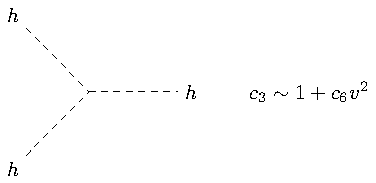
\includegraphics[]{Images/c3.pdf}}\\
There are other three operators which are CP-odd, e.g. $H^\dagger HW_{\mu\nu}\Tilde{W}^{\mu\nu}$. All these operators affect only the Higgs physics and can modify the Higgs coupling, so if we have the linear Lagrangian the modification to the Higgs coupling arise at the dimension 6 level. However, we get corrections also from $D=8$ operators. For example, we can consider:
\[
O_{2H}=H^\dagger H[\partial_\mu(H^\dagger H)]^2
\]
Clearly, this operator will give us a shift in the Higgs coupling:
\[
c_v=1-\frac{c_Hv^2}{4}+c_{2H}v^4+(\cdots)v^6+(\cdots)v^8+\cdots\marginnote{$c_{2H}$ has dimension $-4.$} 
\]
At this point we can understand what is the relation between the linear and non-linear Lagrangian: in the linear Lagrangian, these coefficients scale like:
\[
c_H\sim\frac{g_*^2}{m_*^2} \quad c_{2H}\sim\frac{g_*^4}{m_*^4}
\]
where $g_*$ and $m_*$ are the coupling and the mass characterizing the new physics.\\
The point now is whether such a quantity explode or not and this depends on the scale of new physics. Obviously there are two different possibilities depending on the value of $g_*$ which characterizes the strength with which the Higgs bosons interacts with the new physics, so the stronger this interaction is the more important the corrections will be.\\
In the limit of technicolor, which is a theory in which everything is strongly interacting, this ratio is really of order 1, there is no hierarchy between the numerator and the denominator. If the new physics is strongly interacting and all these terms are important, then we cannot really use the linear realization because the cut-off scale is too small compared to $g_*$. In fact, $g_*\sim4\pi$ is exactly what we have if we do not put the Higgs boson. This is the case in which this new physics is strongly interacting and the scale is such that the ratio is really of order 1.\\
Therefore we have to use the non-linear Lagrangian which, in a sense, re-sums all these terms. Such terms are terms in which we expand in powers of $g/m_*$ so this single coupling encodes the effect of all these higher dimension operators. But since we do not have a separation of scales we cannot really expand in the linear regime. Instead, if the cut-off of the new physics appears at a scale which is large enough and weakly coupled then at this point it will be possible to truncate this series because the higher in the dimension we go the more suppressed the effects will be.\\
It is important to say something about how strong the new physics is, not just at which scale it appears but also if it is strongly or weakly coupled. Strongly coupled physics at small energy implies that the linear realization does not occur. Linearly realized symmetry instead requires a gap and the new physics remains weakly coupled up to the cut-off scale, there is a regime in which the theory is weakly coupled. Of course some of these dimension 6 operators will involve more derivatives and they will map into operators, in the non-linear Lagrangian, involving more derivatives.\\
This is not easy to digest but it is important to do it because there are these two mathematical descriptions and now we have to describe data, so we have to know how to use these descriptions. Depending on the data, one of the descriptions might be good and the other might not be useful. In particular, if the new physics was technicolor then we should have used the non-linear Lagrangian because there was no possible expansion in the linear formalism. On the other hand, if there were no evidence of technicolor then the linear Lagrangian would be a good description.\\
Remember that this is an EFT, so we integrate out the heavy physics and match the full theory with the heavy theory. This gives us the value of $\alpha_T$ and other parameters at the scale we are doing matching, at least at high scale $\alpha_T$ has to be small. What does it mean that it is small at the cut-off scale? It means that the degrees of freedom we are integrating out respects custodial symmetry, the new physics has to be custodial invariant. Here the situation is better at the linear level because custodial symmetry already appears as accidental. As long as there is a gap between the energy at which we do experiments and the cut-off scale then this effect is automatically small but we might be in the other situation and not getting the benefits of accidental custodial symmetry, we have to somehow impose it at the level of the new physics. Notice that the presence of this term is exactly what differentiates the two possible different patterns of global symmetry breaking.
\[
\begin{aligned}
&\alpha_T=0: &&\text{SU$(2)_{\text{L}}\times$SU$(2)_{\text{R}}\to$SU$(2)_{\text{V}}$}\\
&\alpha_T\neq0: &&\text{SU$(2)_{\text{L}}\times$U$(1)_{\text{Y}}\to$U$(1)_{\text{EW}}$}\\
\end{aligned}
\]
These two possibilities correspond to two different patterns of global symmetry breaking. Both patterns will give us 3 NGBs which will have to transform, as usual, as the representation of the unbroken group. In the first case, the 3 NGBs are 3 irreps, so an adjoint of SU$(2)_{\text{V}}$. In the second case instead, they are reducible representations denoted by $\chi^\pm$ and $\chi^0$ and that is why we can write two kinetic terms, one for each reducible representation. If we enlarge the pattern of symmetry breaking, for example at the classical level, and if we include the Goldstone bosons that come from the spontaneous breaking of U$(1)_{\text{A}}$\marginnote{Forget for a moment about the anomaly.} then we will have two kinetic terms with two unrelated coefficients. This is important in the limit of large number of colours because in that case the anomaly switches off. Every time the Goldstone bosons form reducible representations, with respect to the broken group, then each reducible representations has its own kinetic term. The fact that experimentally the custodial symmetry is an approximate symmetry of our world implies that up to small effects these 3 NGBs are transforming very closely to an irreducible representation of SU$(2)_{\text{V}}$, that is the custodial symmetry. 
\section{Scattering Amplitudes at High Energies}
Before discussing the Higgs physics and how the Higgs boson decay we want to analyze a bit what happens to the scatterings for generic Higgs couplings. We have said that this theory is effective, is not a complete one and this means that there must be some process whose cross section blows up when we go at high energy so the theory cannot be maintained at perturbative regime. Which scattering amplitudes should we consider? Let's first analyze the role of the coupling $c_v$ which corresponds to two vector bosons going to one Higgs.\\
\begin{figure}[h]
    \centering
    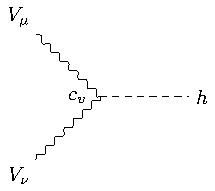
\includegraphics[width=0.4\textwidth]{Images/cvvv.pdf}
    \caption*{}
    \labfig{cvvv}
\end{figure}\\
We should remember from the previous course\marginnote{Previous course=\cite{EW}.} that the exchange of the Higgs in the $WW$ scattering amplitude was crucial to restore perturbative unitarity, so one amplitude that we should monitor is $W^+W^-\to W^+W^-$.\\
\begin{figure}[h]
    \centering
    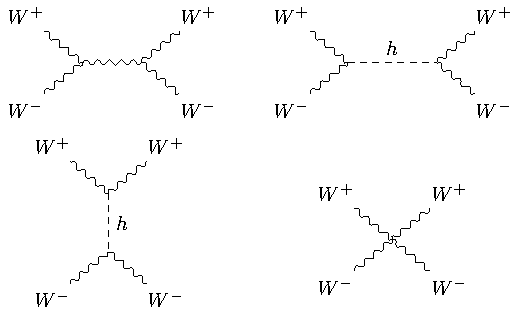
\includegraphics[width=0.8\textwidth]{Images/wwww.pdf}
    \caption*{}
    \labfig{wwww}
\end{figure}\\
The total amplitude goes like:
\[
A=\frac{1}{v^2}\left[s-\frac{s^2}{s-m_h^2}c_v^2+(s\leftrightarrow t)+\cdots\right]\underset{\mathclap{\tikz \node {$\uparrow$} node [below=1ex] {\footnotesize  $s\to\infty$};}}{\simeq}\frac{s}{v^2}(1-c_v^2)+(s\leftrightarrow t)+\cdots
\]
There is a contribution which grows with the energy coming from the sum of the pure $W$ diagrams, and it is the term $s/v^2$, but then there is the contribution from the Higgs exchange with the $c_v^2$ factor coming from the fact that there are two couplings. The $\cdots$ denote finite terms which do not grow with the energy. If we want to cancel this growth with the energy, we have to set $c_v=1$, that is the way to cure the loss of perturbativity. This is the Standard Model point, it is a bottom-up way to derive the SM.\\
Then there is also the coupling $c_{2v}$, the coupling of two Higgs with two $W$. In order to constrain that, we have to consider the following scatterings processes.\\
\begin{figure}[h]
    \centering
    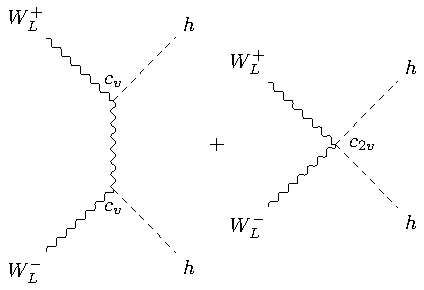
\includegraphics[width=0.6\textwidth]{Images/wlh.pdf}
    \caption*{}
    \labfig{wlh}
\end{figure}\\
At high energy, this amplitude goes like:
\[
A\simeq\frac{E^2}{v^2}(c_{2v}-c_v^2)+\cdots
\]
Again, we have to set $c_{2v}=1$ in the SM so that the amplitude does not explode. Why does the sum of these terms go like $E^2$? Because the polarization goes like one power of the energy, $\varepsilon_\mu^L=\frac{p_\mu}{m_W}(1+\pazocal{O}(m_W^2/E^2))$. We have two of these objects, the coupling has no derivatives so the amplitude goes like $E^2$.\\
In this story it is very useful to use the equivalence theorem, which tells us that we can simplify the calculation by replacing the longitudinal $W$ with the would-be Goldstone bosons which interact with the Higgs through the chiral Lagrangian when we switch off the gauging. For example for this process we have:\\
\begin{figure}[h]
    \centering
    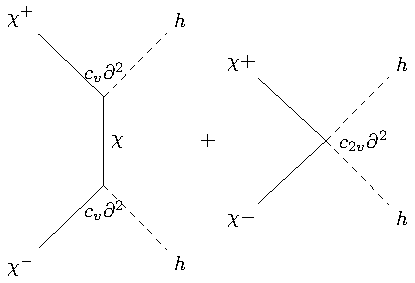
\includegraphics[width=0.7\textwidth]{Images/chih.pdf}
    \caption*{}
    \labfig{chih}
\end{figure}\\
Now, there is no energy factor coming from the polarization vector but there are derivatives in the vertices. The diagram on the left in particular gives four powers of the energy from the vertices, $1/v^2$ from the propagator so again it is proportional to $v^2$ and there are two powers of $c_v$. The simplification we get by using the equivalence theorem is more evident if we look at $WW$ scattering where there is sum over diagrams involving only the $W$ bosons and the equivalence theorem maps everything into just one diagram where the vertex goes like two derivatives. Here the equivalence theorem is very useful because each diagram naively goes like $E^4$ since there are 4 longitudinal $W$. For the diagram relative to the contact interaction this is easy to see, for the process with the propagator there is a factor $E^4$ coming from polarizations, $E^2$ coming from the vertices and then the propagator which in the unitary gauge goes like $E^0$ so in the end it will go like $E^6$. However, if we sum all these diagrams then we find that there is a cancellation and this sum goes like $E^4$. Now if we sum everything, the total goes like $E^2$ because there is another cancellation. In addition to that, we have to add the contribution of the Higgs which goes like $E^2$ so in the SM there would be another cancellation. It is clear that all this calculation would be way easier by using the equivalence theorem. When we want to use these tools to parametrize the Lagrangian, we keep the couplings $c_v$ and $c_{2v}$ generic and there would be no cancellation in the diagrams involving interactions between the Higgs and the $W$.\\
In order to constraint the coupling $c_q$, we look at the scattering of $W$ bosons into quarks, i.e. $W_L^+W_L^-\to q\overline{q}$.
\begin{figure}[h]
    \centering
    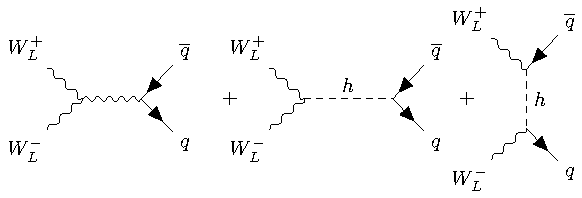
\includegraphics{Images/wwqq.pdf}
    \caption*{}
    \labfig{wwqq}
\end{figure}
There is a factor $E^2$ coming from the $W$ bosons, there is a $\sqrt{E}$ coming from each spinor and in the unitary gauge there is no derivative so it will be proportional to a factor $m_q/v^2$ and finally $1/E^2$ coming from the propagator so this diagram goes like:
\[
E^2(\sqrt{E})^2\frac{m_q}{v^2}\frac{1}{E^2}\sim E\frac{m_q}{v^2}
\]
The growth is not like $E^2$ but instead is proportional to one power of the energy times the mass of the quark which means that in order to better see this effect we should consider the top quark. Using the equivalence theorem, we obtain an interaction involving $\Sigma$, $q$ and also the Higgs. By expanding $\Sigma$, which is $\exp{i\chi^a\sigma^a/v}$ then we get:
\[
\overline{q}_L\Sigma q_R\left(1+c_q\frac{h}{v}+c_{2q}\frac{h^2}{v^2}+\cdots\right)\simeq\overline{q}_Lq_R(1+\chi+\chi^2+\cdots)
\]
This is a contribution which couples directly two $\chi$ with $q\overline{q}$ and goes like $m_q(\sqrt{E})^2/v^2$. Notice that these quarks have opposite helicity, of course there are different scatterings, e.g. we can consider $\chi\chi\to q_Lq_R$ or $\chi\chi\to q_Lq_L$ or $\chi\chi\to q_Rq_R$. The process which goes like $E^2$ is the one involving left- and right-handed.\\
There is a left-right invariance of the chiral Lagrangian under which we exchange left- and right-handed. At the level of $\Sigma$, the axial generators in the exponential get a minus sign and we can also say the same thing by transforming the fields instead of the generators so under this symmetry $\chi\to-\chi$. The vertices which come out of this interaction have to involve an even number of $\chi$ bosons. The possible diagrams are then given by:
\begin{figure}[h]
    \centering
    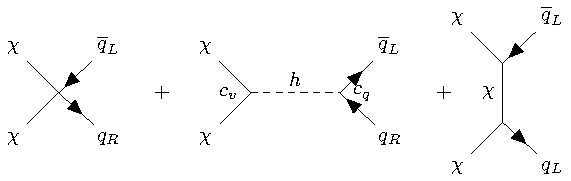
\includegraphics{Images/chichiqq.pdf}
    \caption*{}
    \labfig{chichiqq}
\end{figure}\\
Looking at the amplitude of the diagram on the right, this goes like $(\sqrt{E})^21/E\sim E^0$ and as we can see it does not grow with the energy. If we select the scattering of $\chi\chi$ going into two left-handed quarks then the amplitude does not grow with the energy, if we select instead left- and right-handed quarks then we will get something which grows like $E$. But there is also a contribution from the Higgs with an amplitude going like $E^2(\sqrt{E})^21/E^2$. Summarizing, using the equivalence theorem in the $\xi$-gauge we are left with the contributions of the first two diagrams, i.e. $\chi\chi\to\overline{q}_Lq_R$.
\[
A(\chi^+\chi^-\to\overline{q}_Lq_R)\propto\frac{m_qE}{v^2}(1-c_vc_q)+\cdots
\]
This has to be 0 in the SM, which implies that $c_q=1$ since we already constrained $c_v$ to be equal to 1.\\
There are other couplings that we can consider, for example the triple Higgs coupling. This coupling by itself does not involve a growth with the energy in the scattering amplitude, it does not give any problems because there is no cancellation in scattering amplitudes which is ruined by this parameter. There are other interactions instead more problematic, e.g. we can look at $c_{2q}$ which is the coupling of $q\overline{q}$ with two Higgs.
\begin{figure}[h]
    \centering
    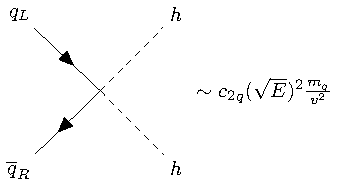
\includegraphics[width=0.6\textwidth]{Images/c2q.pdf}
    \caption*{}
    \labfig{c2q}
\end{figure}\\
It is not something that can be easily done experimentally but it exists on the theoretical side. If $c_{2q}$ was different from zero it would create a growth with the energy so we have to impose that $c_{2q}=0$ because otherwise there is a single contribution from this scattering which grows with the energy.\\
The fundamental question is: \textit{how much can we extrapolate of a theory given the knowledge of the precision that we have on the Higgs couplings?}\\
The precision on the Higgs coupling is:
\[
\frac{\delta g_h}{g_h}\approx10\%
\]
This number is an over-simplification, there are some couplings which are better and other couplings which are not even known. As we will see, it depends on how we do the fit. We have a certain set of experimental data that we have to fit with some theoretical predictions and this depends on how many assumptions one makes. For example, if we make a super generic fit then there will be so many couplings that we will not be able to fit so there is the need to make some simplifications. One possible simplification is the one in which one says \textit{okay let me consider the possible situation in which are the couplings are shifted by a single common parameter}, e.g. if the only operator we turn on is $O_H$ that is exactly the case, a universal shift to all the couplings. The precision that we get on this deviation is better than 10\%, is (4-5)\%. In this picture, we have that at the electroweak scale $\pazocal{O}(100$\,GeV) we can extrapolate the theory up to which point? Suppose we take any of these couplings and make them different from the SM prediction, what do we get? An amplitude which goes like:
\[
A(WW\to WW)\propto\frac{E^2}{v^2}(1-c_v^2)\simeq\delta c_v\frac{E^2}{v^2}\Rightarrow E\lesssim\Lambda=\frac{4\pi v}{\sqrt{\delta c_v}}
\]
This is because perturbative unitarity is loss when the amplitude is of order of $16\pi^2$. The theory will become non-perturbative and non-unitary at this scale and new physics has to come essentially before this scale. It is then possible to extrapolate up to energy of this order. If we assume $\delta c_v$ of order 10\% then we get $\Lambda\approx10$\,TeV. The answer is that the knowledge we have on these couplings justifies the extrapolation of the theory up to energy of order 10 TeV in a weak regime. If the couplings are closer to the SM predictions then perturbative unitarity holds true for longer and the sooner new physics appear, the weaker can be.\\
It is possible to repeat the story for a theory without the Higgs, in this case there will be $\Lambda=4\pi v$ and scattering amplitudes at this scale will blow up. New physics has to come before $\Lambda$ and in this case it would be the Higgs, in fact when they were looking for the Higgs before its discovery they did not know where the mass was and they were saying \textit{okay, if the Higgs is as far as 1 TeV it is so heavy that the theory is very strongly coupled}. It turned out that the Higgs was lighter so the theory is weakly coupled.\\
In the SM point, in principle we can extrapolate the theory to very very high energies without having problems with scattering amplitudes however the couplings will run logarithmically and again we might have a loss of perturbativity due to the fact that some of the couplings blow up. There are two possible couplings which can blow up: the quartic coupling of the Higgs and the one relative to the hypercharge.\marginnote{The point is that it blows up at $10^{42}$\,GeV so we do not care.}  Consider now the SM, which has a potential given by:
\[
V(H)=-\mu^2(H^\dagger H)+\lambda(H^\dagger H)^2
\]
The coupling $\lambda$ will have contributions from itself and from the top quark:\marginnote[-1cm]{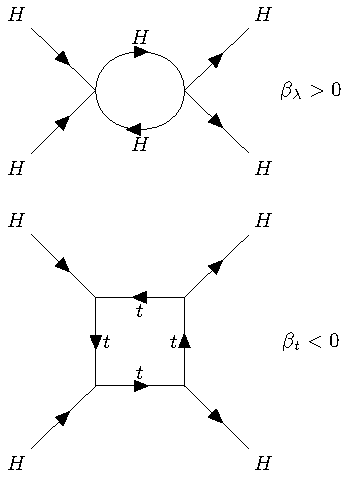
\includegraphics[]{Images/betatbetal.pdf}\\
Contributions for $\beta_\lambda$ and $\beta_t$.}
\[
\mu\frac{d}{d\mu}\lambda=\frac{\beta_\lambda}{16\pi^2}\lambda^2+\frac{\beta_t}{16\pi^2}y_t^4
\]
$\beta_\lambda$ is positive but $\beta_t$ is negative. Notice that $\lambda$ morally is the coupling squared, loss of perturbation theory occurs for $\lambda$ of order $16\pi^2$. There are two compelling effects in this story and it depends on the initial condition: if we start with a very small value of $\lambda$, i.e. light Higgs, then the first term would be subleading with respect to the top term which will win and the coupling will decrease as we go up in energy. On the other hand, if $\lambda$ at the initial point is large, i.e. heavy Higgs, then the first term will dominate, the coupling will increase by running up in energy and perturbative unitarity will be lost at a certain point. It turns out that the Higgs is light so the first term is subleading, the initial conditions are so small that the top ends up winning. The coupling decreases with the energy and there is a very very high energy at which $\lambda$ crosses the zero and becomes negative. One might now be worried that a negative $\lambda$ corresponds to a potential which is unbound from below.\marginnote{There is a connection between the evolution of $\lambda$ as a function of the energy and the stability of the vacuum, but it is a bit technical so I will skip it.}
%La roba a bit technical sta da 1:27:43 in poi lezione del 05/12
\section{Higgs Physics at LHC: an Overview}\marginnote{All the plots in this section come from these slides (\href{https://drive.google.com/file/d/1nRTaJiSPKT-3GF6tWTK1DD527NBhDl-t/view}{pdf}, \href{https://docs.google.com/presentation/d/1rkPtbXIJHBdueZSCO1WJ5AldcSCCZvTq/edit?usp=sharing&ouid=116478279443568847759&rtpof=true&sd=true}{ppt}) which can be found on the \href{https://sites.google.com/uniroma1.it/wismb2223/home}{course website}.}
\subsection{Production}
How can we produce a Higgs boson? It has to come from the interaction of particles with sufficiently high energy. At LEP they tried with $e^+e^-\to Zh$,
% \begin{figure}[h]
%     \centering
%     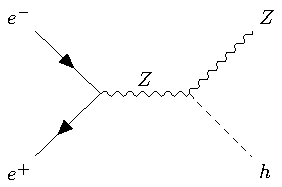
\includegraphics[width=0.45\textwidth]{Images/higgslep.pdf}
%     \caption*{}
%     \labfig{higgslep}
% \end{figure}\\
this process requires having an invariant mass of $\sqrt{s}>m_h+m_Z$ and there was not enough energy to make it happen. At LHC more energy was available but it is a much more complicated environment: basically protons are smashed together. Protons are composite particles made of three quarks as we know and $\sqrt{s}$ was 7 TeV at the time of the discovery, then it went up to 8 TeV and finally to 13 TeV. The first two values correspond to Run 1, the latter to Run 2. Run 3 just started with increased energy but analyzed data from Run 3 are not available yet, so the results will come from Run 1 and Run 2 and we will consider the integrated luminosity of Run 2 much larger than the one of Run 1.\\
How can the Higgs boson be produced at LHC? It has couplings with the quarks so the process is the following:
\begin{figure}[h]
    \centering
    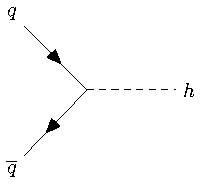
\includegraphics[width=0.35\textwidth]{Images/qqhiggs.pdf}
    \caption*{}
    \labfig{qqhiggs}
\end{figure}\\
However, this vertex is proportional to $m_q/v$ so it is large if we have the top quark but unfortunately the top quark is not one of the valence quarks. But in addition to the valence quarks there are also the sea quarks, i.e. quarks that are produced by fluctuations in the vacuum coming from the facts that these quarks radiate  virtual gluons which split and in principle it is possible to have everything. We can even think of having a top out of this but it is very difficult, it has a very small probability to happen. Creating a bottom is more feasible, the probability of having a bottom inside a proton is not entirely negligible. It turns out that at the energy of the LHC, the probability to get a gluon inside the partons is very large, so one of the main process that it is possible to have is \textbf{gluon-gluon fusion} (GGF). These two gluons can meet and interact: 
\begin{figure}[h]
    \centering
    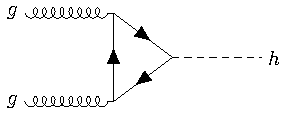
\includegraphics[width=0.45\textwidth]{Images/ggf.pdf}
    \caption*{}
    \labfig{ggf}
\end{figure}\\
In the loop, the top quark will give the largest contribution. Despite the fact that this is a one-loop effect, it gives the largest cross section at LHC.\\
Then there is the coupling with vector bosons, however extracting the $W$ from the proton is difficult and very very rare. We then start with quarks and radiate a $W$ from the quarks, so the process which goes under the name of \textbf{vector boson fusion} (VBF) is:
\begin{figure}[h]
    \centering
    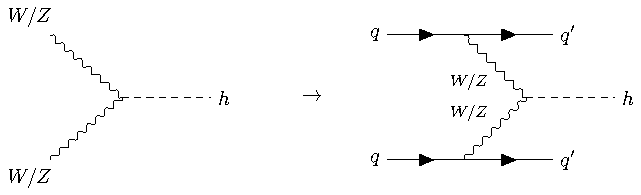
\includegraphics[width=0.8\textwidth]{Images/vbf.pdf}
    \caption*{}
    \labfig{vbf}
\end{figure}\\
Here the final state is not just the Higgs but the Higgs plus two quarks and it turns out that these quarks are very forward. Normally we have an interaction along the $z$-axis and the products in the final state have a certain distribution but particles that are very close to the beam line are more difficult to detect because there is other stuff which goes forward: two quarks can interact but the rest of the protons travel and hit the detector as well in the forward direction. It is much more clean to look at what happens in the transverse direction.\\
VBF has a cross section which is way smaller than GGF because we need to have a $W$ or $Z$ boson radiated from the quarks, there are couplings involved. It is true that in GGF there is a loop but the couplings are strong and they are larger than the ones in VBF.\\
There is also associated Higgs production which is when we have $q\overline{q}\to W/Zh$:
\begin{figure}[h]
    \centering
    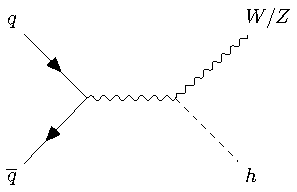
\includegraphics[width=0.4\textwidth]{Images/higgsprod.pdf}
    \caption*{}
    \labfig{higgsprod}
\end{figure}\\
Here it has to be $Z$ when the initial state is neutral, so final state has to be neutral as well, but it could be a $W$ when the initial state is charged, e.g. when we have $u\overline{d}$. At LHC, $\overline{q}$ is a sea quark, i.e. not one of the three valence quarks, it comes from fluctuations of the vacuum of a virtually produced gluon. Associated Higgs production is again less frequent than GGF. Finally, there is another process which uses the coupling with the top:
\begin{figure}[h]
    \centering
    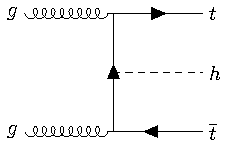
\includegraphics[width=0.4\textwidth]{Images/tth.pdf}
    \caption*{}
    \labfig{tth}
\end{figure}\\
The price to pay is that the top appears also in the final state of other processes so it is possible to have the gluons and then a $t\overline{t}$ pair to which we attach the Higgs. This is $t\overline{t}h$ production which requires a very large $\sqrt{s}$ so its cross section is one of the smallest ones.\\
\marginnote[-2cm]{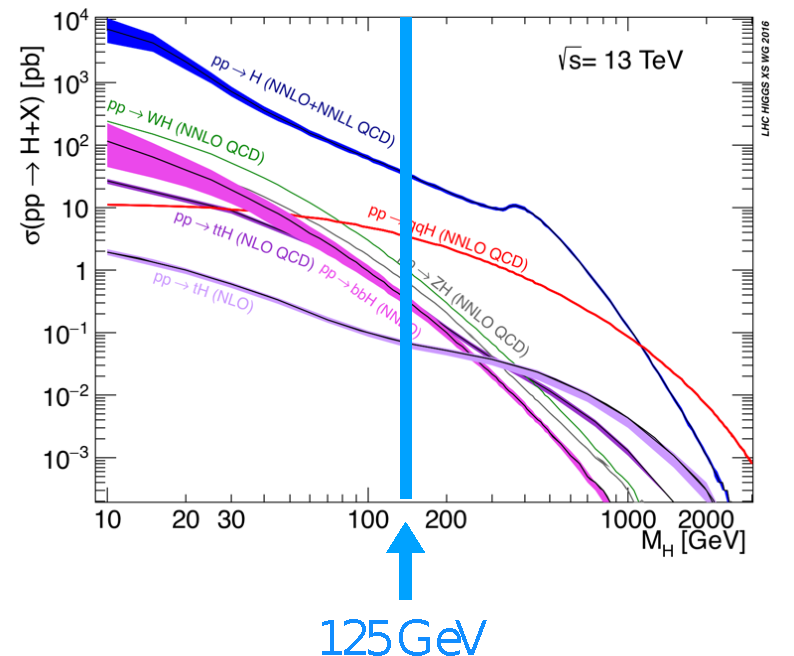
\includegraphics{Images/higgsplot.pdf}\\NNLO is the Next to Next Leading Order and represents some important corrections.}In the plot on the side, a summary of the various cross sections for different values of $m_h$ is shown. The Higgs mass is 125 GeV so we should look at the hierarchy highlighted by the cyan arrow. The total cross section is the sum of all cross sections of these processes and at $\sqrt{s}=13$\,TeV it turns out to be 56 pb. How many Higgs bosons are produced at LHC? In Run 1 there were something like 70k Higgs bosons while in Run 2 almost a million were produced, 900k. Be careful because these are the ones which were produced, they have to be detected and at this point it depends on how the Higgs boson decay.
\subsection{Decay}
The Higgs boson decays into two quarks $H\to q\overline{q}$ but it cannot go into two tops since $m_t=173$\,GeV$>m_h=125$\,GeV, so the largest decay channel into quarks is $b\overline{b}$. This has a branching ratio of something like 60\%. However, detecting $b\overline{b}$ and distinguishing it from all the other quarks that can be produced at LHC is a very difficult challenge. These quarks transform themselves into jets and when the energy decreases they start to form hadrons. This transition is called \textbf{hadronization}, some hadrons can be unstable and they will decay.\\
What are the other possible processes? The Higgs cannot go into two $W$ but one of the two can be virtual and can decay either in $l\overline{\nu}$ or $q\overline{q}$.
\begin{figure}[h]
    \centering
    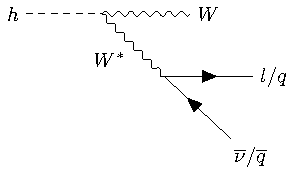
\includegraphics[width=0.45\textwidth]{Images/hd1.pdf}
    \caption*{}
    \labfig{hd1}
\end{figure}\\
The process is then a three-body decay of the Higgs and it has a branching ratio around 30\%. Every time there are quarks things are complicated while with leptons things are easier: the cleanest possibility is when everything is leptonic but then we lose in probability. Another possible decay is the one in which the Higgs goes into two gluons but that is a nightmare because these gluons are submerged by tons of other gluons and quarks but there is a similar process with photons instead of gluons.
\begin{figure}[h]
    \centering
    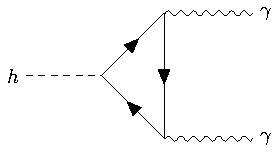
\includegraphics[width=0.45\textwidth]{Images/hphotons.pdf}
    \caption*{}
    \labfig{hphotons}
\end{figure}\\
This is very rare, the branching ratio is 0.2\% but it is very clean because these two photons emerge separately and the invariant mass is 125 GeV. Actually not really clean because there are many many jets which fake photons, so the background we will see is very large and it is not coming from real photons but it comes from jets which eventually leave that energy in the detector and simulate a photon. Photons leave energy in the electromagnetic calorimeter and unfortunately jets do the same, in addition to depositing energy in the hadronic calorimeter. Some of the jets, very rarely, leave a signature which is very similar to the photons. It happens rarely but since we have so many jets there is eventually a significant contribution to the background.\\
One last possible decay process is the one in which the Higgs goes into two $Z$ which then decay each in a pair $ll^+$.
\begin{figure}[h]
    \centering
    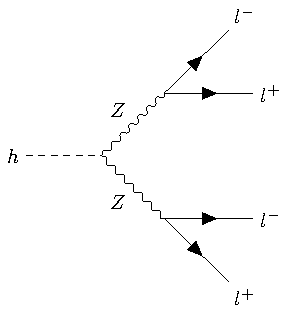
\includegraphics[width=0.45\textwidth]{Images/h4l.pdf}
    \caption*{}
    \labfig{h4l}
\end{figure}\\
Compare it with the situation with the $W$ instead of the $Z$ where there are two charged leptons and two neutrinos and it is not possible to reconstruct the invariant  mass while in this case it is possible to reconstruct both invariant masses and we expect something of 125 GeV. $h\to4l$ and $h\to\gamma\gamma$ were the channels of discovery. A summary of the branching ratios for the different decay channels at $m_h=125$\,GeV is listed in the table below, while in the plot on the side it is possible to see how the branching ratios vary with the Higgs mass.\marginnote[2cm]{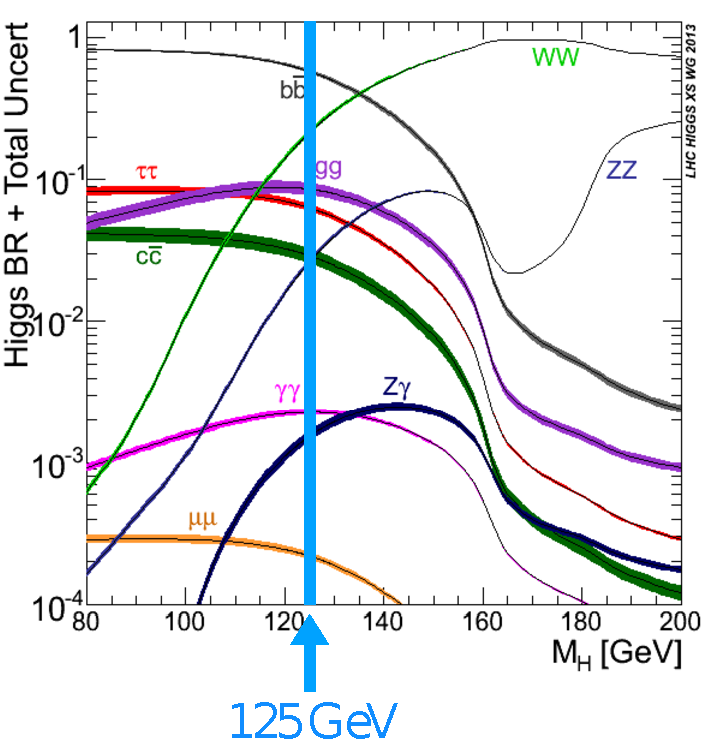
\includegraphics{Images/higgs2.pdf}}
\begin{table}[h]
    \centering
    \begin{tabular}{c|c||c|c}
    \hline
    \rowcolor{gray!45}Process & Branching Ratio & Process & Branching Ratio\\
    \hline
    $b\overline{b}$ & 58\% & gg & 8.2\%\\
    $WW^*$ & 21\% & $Wl\nu$ & 4.6\%\\
    $ZZ^*$ & 2.6\% & $Zll$ & $1.8\times10^{-3}$\\
    $ZZ^*\to4l$ & $1.2\times10^{-4}$ & $\gamma\gamma$ & $2.3\times10^{-3}$\\
    \hline
    \end{tabular}
    \caption{Branching ratios for the different Higgs decay channels ($l=e,\mu$).}
    \labtab{br}
\end{table}\\
Because of its mass, the total Higgs width is very small,  $\Gamma_h=4.1$\,MeV, and the main reason is that the couplings are small.
\subsection{Couplings}
One of the predictions of the SM is that the Higgs coupling with two fermions is proportional to $m_\Psi/v$ and with two vectors is proportional to $m_v/v$. There are these proportionality relations which can be tested. The prediction is for a straight line, as it is possible to see in the picture below.
\begin{figure}[h]
    \centering
    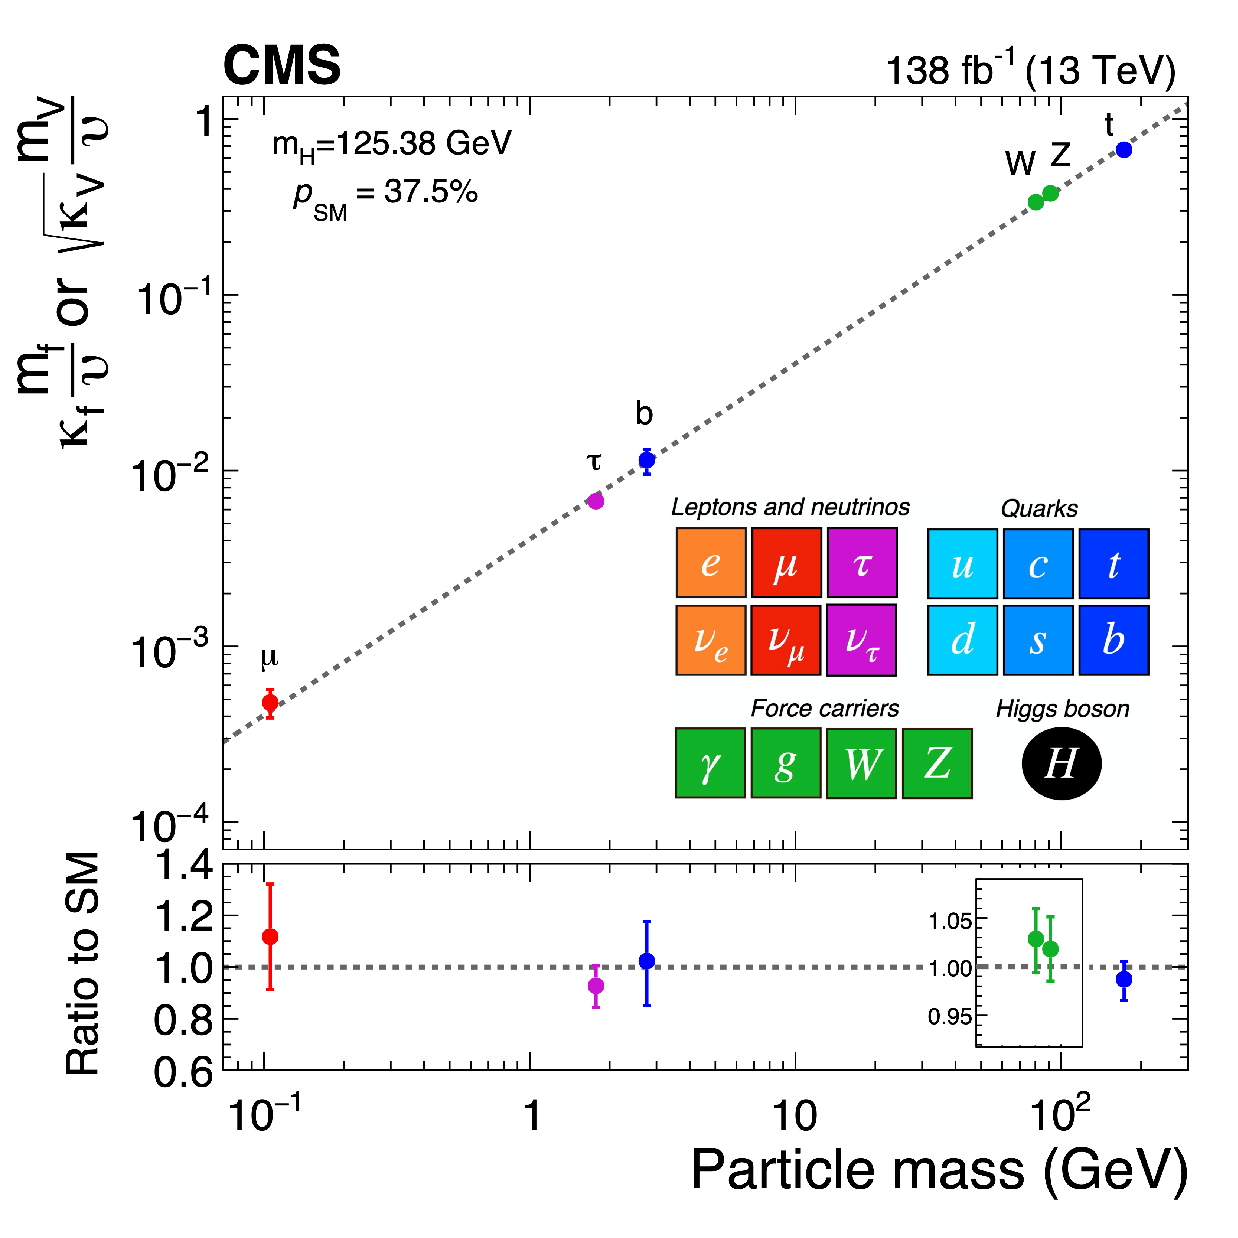
\includegraphics{Images/higgscouplings.pdf}
    \caption*{}
    \labfig{higgscouplings}
\end{figure}\\
Notice how these couplings are so different in strength but they all agree with the SM predictions. It is clear that there is a mechanism which relates the coupling to the mass of the particle.\\
One question is: \textit{which couplings will we eventually observe in nature?} This fit (and other fits made by ATLAS and CMS) are done assuming all the fermions couple in the same way but which couplings can be directly tested? Because some of them are very small and there is no evidence so far. Remember that the existence of the Higgs particle has nothing to do with electroweak symmetry breaking. The latter is just a fact, it generates the $W$ and $Z$ masses and occurs even in absence of the Higgs boson. \marginnote{If we do not include the Higgs boson the theory is effective but we do not really care.} There are models called fermiophobic models in which the Higgs do not couple with fermions and one of the questions that experimentalists tried to answer was whether this particle coupled to the fermions or not. The answer is yes. So far, the coupling with $\tau\tau$ has been discovered and the one with $b\overline{b}$, in the different channels previously presented. Moreover, it has also been observed the $tth$ production and CMS reported evidence of the Higgs coupling with $\mu\mu$. 
\subsection{Double Higgs Production}
A lot of studies now focus on double Higgs production because there is still no evidence of the Higgs self interaction, that coupling has not been measured. The cross section of this process is way smaller compared to the ones we have seen before, at 14 TeV it is a thousand times smaller than single Higgs production, $\sigma(pp\to hh)=45$\,fb. 
\begin{figure}[h]
    \centering
    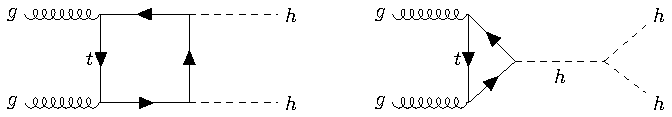
\includegraphics[width=0.8\textwidth]{Images/doublehiggsprod.pdf}
    \caption*{}
    \labfig{doublehiggsprod}
\end{figure}\\
There is now GGF with a box loop and two Higgs or the cubic interaction, there is single production but the Higgs is produced virtually and it splits into two final Higgs. It turns out that these two diagrams, unfortunately, interfere destructively. What is possible to do is varying the cubic coupling obtaining a drastic change in the cross section, so if there is new physics it will modify the cubic interaction. To detect this Higgs pair, one promising channel is $hh\to b\overline{b}b\overline{b}$ because there are a lot of expected events, very difficult to detect but experimentalists derive strategies which can be useful.\\
Also with double Higgs production it is possible to plot things as a function of the invariant mass because there could be some heavy Higgs which is produced in some way which can then decay into $hh$. This is possible, there are many models in which this happens and it will increase the double Higgs production cross section. The mass of $hh$ will resonate at the value of the mass of the heavy Higgs so when we study the invariant mass distribution of the double Higgs production we can look for bumps. There are many studies which search for heavy Higgs in this way. When looking at double Higgs production searches there are two types: resonant and non-resonant. The one we discussed here is resonant, there is a production of a particle which then decays into two other ones. In these case, performing the analysis is easier while in the non-resonant double Higgs production, which is the SM one, there is no intermediate on-shell particle.  
\section{The Standard Model with $v\ll\Lambda_{\text{QCD}}$}
Now we take a look at the possible situation in which $W_L$ and $Z_L$ are not elementary but composite, which is realized in technicolor theories. It also realizes in theories where the Higgs field is a composite one. In the SM these particles are not composite, because they come from the Higgs field which is elementary, is a fundamental field. The 3 degrees of freedom of $W_L$ and $Z_L$ are elementary in the SM.\\
However, we can imagine a world in which we change the value of the vacuum expectation value $v$ of the Higgs: instead of being 246 GeV we decrease it. The theory will now undergo a Higgs mechanism at a scale $v$ which is smaller than $v_{\text{SM}}$. At this scale, the theory is weakly coupled and consequently the coupling will be larger than it is in the SM. If we continue going down, there will be a certain point at which the Higgs coupling will be so large that the theory will confine. There is a dynamical scale $\Lambda_{\text{SU}(2)}$ at which SU$(2)_{\text{EW}}$ confines. If $v$ is smaller than $\Lambda_{\text{SU}(2)}$ then the situation is not quite the one that we know because the coupling will become so strong that before the Higgs mechanism takes place there will be confinement like in QCD, it is a completely different theory. There is another important scale, $\Lambda_{\text{QCD}}$, at which QCD confines. We know that $\Lambda_{\text{QCD}}>\Lambda_{\text{SU}(2)}$ because of the values of the couplings.\\
Now we want to see the case where:
\[
\Lambda_{\text{SU}(2)}\ll v\ll\Lambda_{\text{QCD}}
\]
Why do we want to study this? When QCD happens, condensate of quarks $q\overline{q}$ forms and this condensate is not a singlet under SU$(2)\times$U(1) since it is between one left-handed and one right-handed quark. This corresponds to a bilinear operator called $O$, a composite scalar field and condensation means that it acquires a vev $\Braket{O}$. That is the order parameter which breaks chiral symmetry. Because physical meaningful quantities are gauge invariant and here we are talking about colour, this has to be a colour singlet. This vev is proportional to $\Lambda_{\text{QCD}}^3$. Why are we confident that this vev exist? Forget for a moment about electroweak interaction and look at QCD with just 2 flavours, up and down. This theory of two flavours has chiral symmetry in the Lagrangian.
\[
\pazocal{L}_{\text{QCD}}=-\frac{1}{4g_3^2}G_{\mu\nu}^aG^{\mu\nu,a}+\overline{q}(i\slashed{D}-m_q)q
\]
The kinetic term has an SU$(2)_{\text{L}}\times$SU$(2)_{\text{R}}$ invariance for $m_q=0$, that is an accidental global symmetry in this theory which gets explicitly broken by the mass term $m_q\propto\mathbb{1}$. SU$(2)_{\text{L}}\times$SU$(2)_{\text{R}}$ is broken to SU$(2)_{\text{V}}$, this is really the vectorial subgroup by definition\marginnote{The vectorial subgroup is by definition is the largest subgroup which we can preserve by giving mass to all the fermions.} and in QCD is called \textbf{isospin}. Isospin breaking comes because $m_u\neq m_d$, that is a difference of a few MeV which is much smaller than $\Lambda_{\text{QCD}}\approx$\,a few hundred MeV. If we switch off the mass, this vev will also break SU$(2)_{\text{L}}\times$SU$(2)_{\text{R}}$ but now spontaneously to SU$(2)_{\text{V}}$.\\
There is an explicit breaking from the masses, which is a small effect, and a spontaneous breaking from quark condensate which gives 3 NGBs resulting from the 3 broken generators. These particles in the spectrum are the pions, they have a mass which is much smaller than $\Lambda_{\text{QCD}}$.\marginnote{$m_{\pi^\pm}=139$\;MeV and $m_{\pi^0}=135$\;MeV.} They are light particles because if we switch off the mass term they are massless, they are actually pseudo-NGBs because $m_q\neq0$.\\
At this point, one may object \textit{hey this is not a QCD course why are we doing all of this I'm calling the police}, but this is important for weak interactions because now we can switch on the electroweak gauging which gives a subgroup of SU$(2)_{\text{L}}\times$SU$(2)_{\text{R}}$. Up and down left-handed particles are a doublet of SU$(2)_{\text{EW}}$ and in this story they are a doublet of SU$(2)_{\text{L}}$, it is the same of QCD. Hypercharge is just the third component of SU$(2)_{\text{R}}$ so if we switch on the gauging there is a Higgs mechanism in which these NGB are eaten to form $W_L$ and $Z_L$, hence they will be composite particles because the pions are composite.\\
In principle there are 4 quark condensates which we can consider and they all have to be colour singlet. Let's switch off electromagnetic interactions, this is reasonable since at the QCD scale electromagnetism can be considered as a small perturbation. 
\[
\begin{aligned}
    &\langle\overline{u}_Lu_R\rangle &\langle\overline{d}_Ld_R\rangle\\
    &\Braket{\overline{u}_Ld_R} &\langle\overline{d}_Lu_R\rangle
\end{aligned}
\]
There is a theorem by Vafa and Witten which states that \textit{the vectorial subgroup of the global symmetry G cannot be broken spontaneously in a vector-like gauge theory.}\\
In this statement there are two important assumptions: the first one is that we are in a gauge theory, so there are no additional interactions like the Yukawa ones and this is true in the situation we are considering since we have switched off everything but QCD, and the second one is that the theory is vector-like, which again is true for QCD. For example, in this case we can give the same mass to everybody, with a mass matrix $M$ proportional to the identity, then SU$(2)_{\text{L}}\times$SU$(2)_{\text{R}}$ is explicitly broken to SU$(2)_{\text{V}}$ by this mass matrix. In this situation, the largest unbroken group is SU$(2)_{\text{V}}$. If we give different masses to up and down quarks then we reduce SU$(2)_{\text{V}}$ to U(1).\\
We can also consider a situation where we have fermions $\Psi$ which are real representations of the global symmetry group and we will have SU$(N)\to$SO$(N)$. The mass term will be a Majorana mass term of the form $\Psi_i^\alpha M_{ij}\Psi_j^\beta\epsilon_{\alpha\beta}$. There is also the case of pseudo-real representation and in this case the pattern of breaking is SU$(2N)\to$Sp$(2N)$.\\
Remember that here we are in a situation where the masses are zero, however we can always switch them on, set a privileged direction, the vacuum will align in this direction and then we can switch off the masses. It is like spontaneous symmetry breaking where we turn on an external magnetic field which breaks the symmetry to set the direction of the vacuum, then we switch off the field and the vacuum will still point in that direction. Here the mass plays the role of the magnetic field: it gives one direction and the theorem says that the condensate aligns and have the same direction of the mass term. This means that out of the 4 possible condensates, only two will be non vanishing.
\[
\begin{aligned}
    &\langle\overline{u}_Lu_R\rangle=\langle\overline{d}_Ld_R\rangle\neq0\\
    &\Braket{\overline{u}_Ld_R}=\langle\overline{d}_Lu_R\rangle=0
\end{aligned}
\]
In other words, the condensate as a matrix will have a structure of this form:
\[
\Braket{\overline{q}_iq_j}\propto\mqty(\dmat{1,1})
\]
Which SU(2) subgroup is preserved is arbitrary but we can define it in this way, by turning on the masses, identifying a direction and then switching the masses off. This is telling us that in absence of interactions there will be an unbroken SU(2) subgroup. The theory does not imply that there is a non-vanishing condensate, that's a different statement but it tells us that these two condensates must vanish.\\
The next question is: \textit{what happens if we switch on electromagnetic interactions?} In general, it is a dynamical issue. There is an external weak perturbation and we want to see whether there will be a change of alignment in this condensate or not. The discussion of this topic is too technical but the short answer is that as long as the electromagnetic interactions are weak enough nothing changes.\\
In general, there are two sectors in the SM Lagrangian, one is given by the quarks and the other one by the Higgs. Each of these two sectors has an approximate SU$(2)\times$SU(2) global symmetry. 
\[
\left\{
\begin{aligned}
&\text{Quarks:}&&\text{SU}(2)_{\text{L}}\times\text{SU}(2)_{\text{R}}\times\text{U}(1)_{\text{B}}\xrightarrow[f_\pi]{\text{3 NGBs}}\text{SU}(2)_{\text{V}}\times\text{U}(1)_{\text{V}}\\
&\text{Higgs:}&&\text{SU}(2)_{\text{L}}\times\text{SU}(2)_{\text{R}}\xrightarrow[v]{\text{3 NGBs}}\text{SU}(2)_{\text{V}}
\end{aligned}
\right.
\]
The QCD dynamics breaks the quarks symmetry while the Higgs one is broken by the Higgs potential, both breakings result in 3 NGBs. Without the gauging, there would be in total 6 NGBs, 3 elementary ones coming from the Higgs doublet and 3 composite ones from QCD. When we switch on the gauging we explicitly break the quarks global symmetry down to $[\text{SU}(2)_{\text{EW}}\times\text{U}(1)_{\text{Y}}]_{\text{diag}}\times\text{U}(1)_{\text{B}}$ because at this point the gauging couples both to the Higgs, which is charged under this, and with the quarks which are also charged. In absence of the gauging, each sector has its own global symmetry. The gauging acts both on the quarks and on the Higgs at the same time so it is not possible to rotate the quarks and the Higgs separately, they have to be rotated simultaneously in order to have invariance. $\text{U}(1)_{\text{B}}$ is also included, the hypercharge is given by $Y=T_{3R}+(B-L)/2$. This means that 3 out of the 6 NGBs would be eaten by the gauging and the other 3 would become pseudo-NGBs, i.e. they get a mass because their symmetry is explicitly broken. In the standard situation in which $v\gg\Lambda_{\text{QCD}}$ we do an approximation, we just ignore the effect of the condensate, there are then 3 NGBs which gets eaten. Then we go down to $\Lambda_{\text{QCD}}$ where the symmetry has been broken, the quarks have become massive and we would have 3 NGBs, because now we are considering the effect of the condensate, but since the symmetry is explicitely broken by the masses these 3 NGBs are the three pions in the spectrum.\\
This story can be repeated in our approach, so first we consider the theory at $\Lambda_{\text{QCD}}$ and ignore the spontaneous breaking. The gauging eats the three QCD NGBs and leaves the three NGBs of spontaneous breaking uneaten. When we go down in energy, we should consider whether this global symmetry is explicitly broken or not. The answer is yes, it is explicitly broken because of the Yukawa interactions. In general, we can try to deduce the spectrum without describing the theory in these steps. The uneaten NGBs will acquire a mass both because of the Yukawa terms and because of the gauging.\\
In the standard situation, where $v\gg f_\pi$, this translates in the fact that the pions, which are the uneaten NGBs, acquire a mass both because of the quark masses and also there is a radiative corrections coming from the gauge bosons. This is the reason why the mass of the charged pion is larger than the one of the neutral pion, the difference comes from this effect. If we switch the hierarchy between $v$ and $f_\pi$, the NGBs which are eaten will be mostly virtual and the real ones will get a mass from this effect. 
\[
\left\{
\begin{aligned}
&\ket{W_L,Z_L}=\frac{f_\pi}{\sqrt{f_\pi^2+v^2}}\ket{\pi_{\text{QCD}}}+\frac{v}{\sqrt{f_\pi^2+v^2}}\ket{\chi}\\
&\ket{\pi_{\text{phys}}}=-\frac{v}{\sqrt{f_\pi^2+v^2}}\ket{\pi_{\text{QCD}}}+\frac{f_\pi}{\sqrt{f_\pi^2+v^2}}\ket{\chi}
\end{aligned}
\right.
\]
$\ket{W_L,Z_L}$ are the ones that are eaten, $\ket{\pi_{\text{phys}}}$ will remain in the spectrum.\\
In the standard situation, $v\gg f_\pi$, $\ket{W_L,Z_L}$ are eaten and the physical light degrees of freedom which remain in the spectrum are coming mostly from QCD. But if we switch the hierarchy, $v\ll f_\pi$, then the situation is inverted: $\ket{W_L,Z_L}$ are now mostly those of QCD.\\
It is a very good approximation to forget about QCD when describing electroweak symmetry breaking and forget about electroweak symmetry breaking when describing chiral symmetry breaking in QCD. But here we want to cause physical pain to ourselves and describe everything all at once: there is a large global symmetry which gives two sets of NGBs, then by switching on the gauging we obtain linear combinations. This has the advantage that it is possible to switch the hierarchy however we want and at this point we do the calculation of the masses for the $W$ and the $Z$ neglecting electroweak symmetry breaking and focusing only on QCD. This will end up to be qualitatively the right method but with the only problem than $f_\pi$ is ten thousand times smaller than the electroweak scale so quantitatively we will get masses that are ten thousand times smaller than the observed ones, but there is a custodial symmetry and the $\rho$-parameter is 1.\\
Diagrammatically, we can see that they get a mass because the propagator has a pole at some value. How do we compute this propagator? There is an interaction between the gauge bosons, denoted by $V$, and the flavour currents of QCD.%45:41
\begin{figure}[h]
    \centering
    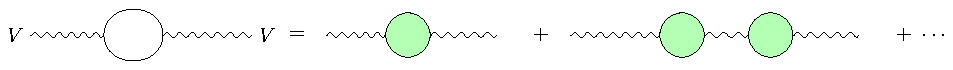
\includegraphics[width=1.5\textwidth]{Images/greenblobs.pdf}
    \caption*{}
    \label{greenblobs}
\end{figure}\\
The green blobs in the diagram above correspond to the two-point function for the currents which the gauge bosons are coupled to. These are the currents of SU$(2)_{\text{L}}\times$SU$(2)_{\text{R}}\times$U$(1)_{\text{B}}$. The hypercharge is coupled to a linear combination of the third generator of SU$(2)_{\text{R}}$ and the current of U$(1)_{\text{B}}$ and the $W$ is coupled to SU$(2)_{\text{L}}$. It is possible to simplify this by forgetting for the moment about U$(1)_{\text{B}}$. This two-point function corresponds to a global symmetry so the two-point function has to be transverse, i.e. if we do the Fourier transform we get:
\[
\Braket{J_a^\mu(p)J_b^\nu(-p)}=(p_T)_{\mu\nu}\delta_{ab}\pi(p^2)\marginnote{This notation denotes the vacuum expectation value of the T-product of the currents.}
\]
where $\pi(p^2)$ is a form factor and $(p_T)_{\mu\nu}$ is given by:
\[
(p_T)_{\mu\nu}=\eta_{\mu\nu}\cdot\frac{p_\mu p_\nu}{p^2}
\]
This is for a given species of currents but we actually have two, left and right, hence three different form factors. 
\[
\Braket{L_a^\mu L_b^\nu}=(p_T)_{\mu\nu}\delta_{ab}\pi_{LL}(p^2) \quad \Braket{R_a^\mu R_b^\nu}=(p_T)_{\mu\nu}\delta_{ab}\pi_{RR}(p^2) \quad \Braket{L_a^\mu R_b^\nu}=(p_T)_{\mu\nu}\delta_{ab}\pi_{LR}(p^2)
\]
However, it turns out that this decomposition is not the most useful one because the vacuum of QCD does not preserve SU$(2)_{\text{L}}\times$SU$(2)_{\text{R}}$ symmetry, it preserves SU$(2)_{\text{V}}$ symmetry. We can then write left and right currents as linear combinations of vectorial and axial currents.
\[
\left\{
\begin{aligned}
&V_\mu=R_\mu+L_\mu\to\overline{q}\gamma_\mu q=\overline{q}\gamma_\mu\frac{1+\gamma_5}{2}q+\overline{q}\gamma_\mu\frac{1-\gamma_5}{2}q\\
&A_\mu=R_\mu-L_\mu\to\overline{q}\gamma_\mu\gamma_5q=\overline{q}\gamma_\mu\frac{1+\gamma_5}{2}q-\overline{q}\gamma_\mu\frac{1-\gamma_5}{2}q
\end{aligned}
\right.
\]
In terms of these new currents, the decompositions now become:
\[
\Braket{V_a^\mu V_b^\nu}=(p_T)_{\mu\nu}\delta_{ab}\pi_{VV}(p^2) \quad \Braket{A_a^\mu A_b^\nu}=(p_T)_{\mu\nu}\delta_{ab}\pi_{AA}(p^2) \quad \Braket{V_a^\mu A_b^\nu}=0
\]
The last one is equal to 0 because of parity: the operator is a product between a vector and a pseudo-vector hence it has the wrong transformation under parity and has to be equal to 0. Necessarily, there is a relation between ($\pi_{LL}$, $\pi_{RR}$, $\pi_{LR}$) and ($\pi_{AA}$, $\pi_{VV}$):
\[
\pi_{LL}=\pi_{RR}=\frac{\pi_{VV}+\pi_{AA}}{4} \quad \pi_{LR}=\frac{\pi_{VV}-\pi_{AA}}{4}
\]
The bare propagator in the $\xi$-gauge is given by:
\[
-\frac{i}{p^2}\left[\eta_{\mu\nu}-(1-\xi)\frac{p_\mu p_\nu}{p^2}\right]=-\frac{i}{p^2}\left[(p_T)_{\mu\nu}+\xi(p_L)_{\mu\nu}\right] \quad \text{where} \;\; (p_L)_{\mu\nu}=\frac{p_\mu p_\nu}{p^2}
\]
The correction coming from the blobs is only a correction to the transverse part, the longitudinal part is not touched but it depends on the gauge so it is unphysical. The resummed propagator is then:
\[
(p_T)_{\mu\nu}\frac{-i}{p^2-g_Ag_B\pi_{AB}(p^2)}+\xi(p_L)_{\mu\nu} \quad A,B=L,R
\]
Does this propagator have any pole for finite values of $p^2$? The poles come only from the transverse part, being the longitudinal one unphysical. For $p^2\to0$, it is possible to expand the form factor in powers of $p^2$. Looking just at the first term, there will be a pole if $\pi_{AB}(p^2=0)\neq0$. The attention is now moved to see whether of this form factors is non-vanishing in 0. Remember that $p_T$ has a pole for $p^2=0$: if there is a non-vanishing value of $\pi_{AB}(p^2=0)$ then this propagator has a singularity at $p^2=0$. But this is not possible because the vector current does not excite any massless state. However, it is the case for the axial current because it excites the pions, which are the NGBs. In other words:
\[
\pi_{VV}(p^2=0)=0 \quad \pi_{AA}(p^2=0)=f^2_\pi
\]
We can verify this by taking an axial current $A_\mu$ which excites a pion that then gets reabsorbed by $A_\nu$. In each vertex the loop is given by the vacuum expectation value between the axial current and the pion field. 
\[
\bra{0}A_\mu(x)\ket{\pi(p)}=if_\pi e^{-ipx}p_\mu
\]
There is then a propagator given by $-i/p^2$ and the contribution for the exchange of the pion is proportional to $f_\pi^2p_\mu p_\nu/p^2$. This implies that:
\[
\pi_{LL}(0)=\pi_{RR}(0)=\frac{f_\pi^2}{4} \quad \pi_{LR}(0)=-\frac{f_\pi^2}{4}
\]
Remember that the $W$ gauges the left current and the hypercharge gauges the right current, so here there is a matrix of possibility: left and right can be chosen in 4 possible ways and this gives a mass matrix.
\[
M_0^2=\left(\begin{array}{cc}
    g^2 & -gg' \\
    -gg' & g'^2
\end{array}\right)\frac{f_\pi^2}{4}
\]
Here, for simplicity, we fixed $a=3$ and in this case there are both left and right. For $a=1,2$ there is no right, $g'=0$ and there is only $g^2$. The one above is the neutral mass matrix but at the same time there is the charged mass matrix:
\[
M_\pm^2=g^2\frac{f_\pi^2}{4}
\]
We now recognize the form of the masses in the SM. There is 0 eigenvalue, i.e. the photon, and then there is another eigenvalue which is the mass of the $Z$.
\[
m_W=g\frac{f_\pi}{2} \quad m_Z=\sqrt{g^2+g'^2}\frac{f_\pi}{2} \quad m_\gamma=0
\]
So the $W$ and the $Z$ have acquired their mass, the photon remains massless and that is exactly the same of the SM with the only difference that instead of $v$ there is $f_\pi$. It is the same because the global symmetry breaking is the same: in the Higgs sector it was SU$(2)\times$SU$(2)\to$SU(2) which is the same in the QCD sector. Moreover, the $\rho$-parameter is equal to 1. In principle, we do not need the Higgs boson to give a mass to the $W$ and the $Z$ bosons: we remove the Higgs from the theory, decrease the energy until we reach the QCD scale and then there are the three NGBs which are eaten. If we compute these masses, they turn out to be $m_W=28$\,MeV and $m_Z=31$\,MeV. The values are not quite correct because we should run the coupling $g$ down to the QCD scale, in this calculation the value of $g$ at a hundred GeV is used.
\section{Technicolor}
As anticipated, the masses we just found are too small but qualitatively everything is okay so this gives us an idea. The idea is to replicate this story by saying that the fundamental Higgs field which gives the electroweak symmetry breaking at 246 GeV is a copy of QCD. Why one should do this perverse complication? Because this UV dynamics does not have a fundamental scalar inside and fundamental scalars imply hierarchy problems. This fundamental scalar has to be much lighter than this UV dynamics but at the moment we do not know the reason why it is like that. For QCD there is no such problem, there are no mass terms of fundamental scalars which we write in the Lagrangian. It is just the Lagrangian of QCD replicated at ten times the energy. This goes under the name of \textbf{technicolor}. Take the SM, remove the Higgs and replace it with the QCD part. The orthogonal combinations of NGBs which are not eaten would remain in the spectrum plus the \nth{4} degree of freedom, the Higgs boson which does not play the usual role of the Higgs boson. These 4 degrees of freedom would be pretty light, the Higgs would have its own usual mass $\mu^2=\lambda^2v^2$ but now $v$ is small. The other three guys, the $\chi$, would have a mass given by gauge interactions and Yukawa terms, which are small effects. By changing parameter, the part of electroweak symmetry breaking now it is coming from QCD dynamics and qualitatively it works, so we can think of technicolor and this was before the Higgs discovery. The other important thing is that a little bit of symmetry breaking comes from the QCD sector but it is so small that is experimentally unobservable , the pions we see in the spectrum are not entirely bound states $q\overline{q}$ but there is a little bit of $\chi$ from the Higgs sector. The fields content and their quantum numbers are very similar to the QCD sector.
\begin{table}[h]
    \centering
    \begin{tabular}{c|ccc}
    \hline
    \rowcolor{gray!45} QCD & SU$(3)_{\text{C}}$ & SU$(2)_{\text{EW}}$ & U$(1)_{\text{Y}}$\\
    \hline 
    $q_L$ & $\Box$ & $\Box$ & +1/6\\
    $u^c$ & $\overline{\Box}$ & 1 & $-2/3$\\
    $d^c$ & $\overline{\Box}$ & 1 & $+1/3$\\
    \hline\hline
    \rowcolor{gray!45}Technicolor & SU$(N)_{\text{Tc}}$ & SU$(2)_{\text{EW}}$ & U$(1)_{\text{Y}}$\\
    \hline
    Q & $\Box$ & $\Box$ & 0\\
    $U^c$ & $\overline{\Box}$ & 1 & $-1/2$\\
    $D^c$ & $\overline{\Box}$ & 1 & $+1/2$\\
    \hline
    \end{tabular}
    \caption*{}
    \labtab{Tc}
\end{table}\\
In the QCD, anomalies of hypercharge are unfortunately non-vanishing so leptons are needed. Technicolor instead is formulated without leptons by choosing judiciously the hypercharges and with the choice shown above this is anomaly free. Technicolor is postulated to conform the condensate at scales much higher than the QCD scale and eventually we have postulated that this scale is the weak scale, $F_\pi=v=246$\,GeV. There would be a global SU$(2)_{\text{L}}\times$SU$(2)_{\text{R}}$ symmetry with respect to the technicolor gauge dynamics and this is broken down to SU$(2)_{\text{V}}$ resulting in 3 NGBs which acquire mass. Everything is the same as discussed in the previous section but instead of $f_\pi$ there is $F_\pi$.\\
Of course this theory has several problems, which we give without going into details since it is probably beyond the goal of this course. In the previous story, the longitudinal $W$ and $Z$ were mostly the QCD pions, i.e. composite degrees of freedom. Here it is the same, they are not elementary fields so when we do the scattering of $W_L$ and $Z_L$ in the spectrum of resonances there would be resonances which we can think of having the same quantum numbers of a Higgs boson but without the right couplings and small width to unitarize the $WW$ scattering. The cross section will eventually grow with $E^2$ and at a certain point we reach the energy of the technicolor scale and discover that these degrees of freedom are composite. The scattering amplitude should not be computed in terms of these bound states but rather in terms of techni-quarks degrees of freedom. In any case, there is an experimental signature, the growth of the $WW$ cross section until the theory becomes non perturbative. There is no Higgs boson in this story, so we expect a very broad resonance. Experimentally, there have been discovered particles with couplings predicted by the SM with excellent precision and for the moment there are no hints that this cross section grows with the energy.\\
Another problem is that this dynamics give a mass to the $W$ and the $Z$ bosons but it does not give a mass to the quarks. By replacing the Higgs sector with the technicolor one, there are still 6 NGBs. We switch on the gauging, the $W$ and the $Z$ acquire a mass but the quarks do not feel the breaking so we need something connecting the quarks with the technicolor sector. This connection goes under the name of \textbf{extended technicolor}. Basically both color and technicolor gauge interactions are enlarged into a larger SU$(N)$ extended technicolor which is postulated to be spontaneously broken at some high energy, so when the heavy extended technicolor gauge bosons are integrated out quarks and techni-quarks will be connected, giving the quarks masses. This mechanism generates four fermions operators which violate flavour so there will be also FCNC.\\
It is possible to conclude that technicolor is excluded by data but it still represents a good class of theories, composite Higgs theories are the modern version of technicolor. 
\section{Electroweak Precision Tests (EWPT)}
As the name suggests, EWPT are tests of the electroweak sector of the Standard Model. The argument is a bit technical so there will be a lot of definition but at the end we will be able to perform a calculation to check if the model satisfies this test or not. The message is that the SM is in very good shape, the EW sector satisfies the test with very good precision. What was to be tested is the genuine EW sector, tests of QED already existed and this program started basically with LEP, at the end of the '80s, when QED was already established. This also sets stringent constraints on everything that comes beyond the SM, every theory that comes beyond the SM has to pass these tests.\\
In the SM there are some parameters which appear in the Lagrangian:
\[
\{g_1, g_2, g_3, \mu^2, \lambda, m_t,\cdots\}
\]
These are the most important ones for EW. It turns out that at tree-level, only 3 combinations of these parameters are important.
\[
\{e,\sin\theta_w,v\} \quad \text{given by}\; \left\{
\begin{aligned}
&\frac{1}{e^2}=\frac{1}{g_1^2}+\frac{1}{g_2^2}\\
&\tan\theta_w=\frac{g_1}{g_2}\\
&v=\sqrt{\frac{\mu^2}{\lambda}}
\end{aligned}
\right.
\]
If we move to loop-level instead there are $\{m_h, \alpha_3, m_t\}$. For each of these parameters we have to find an observable and the most important ones which are very precisely measured are the tree-level ones. EW scheme is a choice of three observables which are used to fix the three input parameters at tree-level. At this point, we do a list of the available observables and choose the three which are more precisely determined.
\begin{table}[h]
    \centering
    \begin{tabular}{c|c}
    \hline
    \rowcolor{gray!45} Observable & Experimental Precision\\
    \hline
    $(g-2)_e\Rightarrow\alpha_{\text{em}}(0)$ & $\sim10^{-9}$\\
    $\mu$-decay$\Rightarrow G_{\text{F}}$ & $\sim10^{-5}$\\
    $m_Z(\delta m_Z\sim2\,\text{MeV})$ & $\sim2\cdot10^{-5}$\\
    $m_W(\delta m_W\sim15\,\text{MeV})$ & $\sim2\cdot10^{-4}$\\
    $m_h(\delta m_h\sim0.9\,\text{GeV})$ & $\sim5\cdot10^{-3}$\\
    \hline
    \end{tabular}
    \caption*{}
    \labtab{obs}
\end{table}\\
One possible choice is $\{\alpha_{\text{em}}(0), G_{\text{F}}, m_Z \}$ but the situation is not as good as it appears. This $10^{-9}$ on $\alpha_{\text{em}}$ is the precision of the measurement at zero momentum. Most of the experiments would be at the $Z$-pole so what we need at the end is to incorporate the electromagnetic corrections which is done by running $\alpha_{\text{em}}$ from zero energy to the mass of the $Z$, hence another possible choice is represented by $\{m_W, G_{\text{F}}, m_Z\}$. How do we measure $\alpha_{\text{em}}$ at the $Z$-pole? At the $Z$-pole, the coupling is given by:
\[
\alpha_{\text{em}}(m_Z)=\frac{\alpha_{\text{em}}(0)}{1-\Delta_\alpha}
\]
where $\Delta_\alpha$ comes from the running. This gets corrections both from leptons and from hadrons:
\[
\Delta_\alpha=\Delta_{\alpha\text{leptons}}+\Delta_{\alpha\text{hadrons}}
\]
The correction coming from hadrons cannot be computed, it has to be extracted from data and in order to do that we use a dispersion relation.
\[
\Delta_{\alpha\text{hadrons}}=\frac{\alpha_{\text{em}}(0)}{3\pi}m_Z^2\text{PV}\int_{4m_\pi^2}^{+\infty}ds\frac{R(s)}{s(s-m_Z^2)}
\]
where $R(s)$ is defined as the following ratio:
\[
R(s):=\frac{\sigma(e^-e^+\to\gamma\to\text{hadrons})}{\sigma(e^-e^+\to l^-l^+)}=\frac{3s}{4\pi\alpha^2_{\text{em}}(0)}\sigma(e^-e^+\to\text{hadrons})
\]
$R(s)$ is then given by this hadronic cross section and it appears here because of the optical theorem. At the end of the day, we get:
\[
\Delta_{\alpha\text{hadrons}}=0.02750\pm0.00033\Rightarrow\alpha_{\text{em}}^{-1}(m_Z)=128.951\pm0.045
\]
with a relative precision of $\sim3\cdot10^{-4}$.\\
The main observables at the $Z$-pole are the total cross section given by $\sigma(e^-e^+\to\gamma,Z\to f\overline{f}+\#\gamma)$, the total $Z$ width and the forward-backward asymmetry defined as:
\[
A_{\text{FB}}:=\frac{\sigma_{\text{F}}-\sigma_{\text{B}}}{\sigma_{\text{F}}+\sigma_{\text{B}}} \quad \left\{\begin{aligned}
&\sigma_{\text{F}}:=\int_0^{+1}d\cos\theta\frac{d\sigma}{d\cos\theta}\\
&\sigma_{\text{B}}:=\int_{-1}^0d\cos\theta\frac{d\sigma}{d\cos\theta}
\end{aligned}\right.
\]
Moreover, there is the $\tau$-polarization:
\[
P_\tau:=\frac{\sigma(\tau_R)-\sigma(\tau_L)}{\sigma(\tau_R)+\sigma(\tau_L)}
\]
All these parameters could be observed both at LEP and at SLC, while only at SLC, where they used polarized $e^-e^+$ beams there were also the left-right asymmetry $A_{\text{LR}}$ and the left-right forward-backward asymmetry $A_{\text{LRFB}}$:
\[
A_{\text{LR}}:=\frac{\sigma(e_L^-)-\sigma(e_R^-)}{\sigma(e_L^-)+\sigma(e_R^-)}\frac{1}{\Braket{P_e}} \quad A_{\text{LRFB}}:=\frac{(\sigma_{\text{F}}-\sigma_{\text{B}})_{e_L}-(\sigma_{\text{F}}-\sigma_{\text{B}})_{e_R}}{(\sigma_{\text{F}}+\sigma_{\text{B}})_{e_L}+(\sigma_{\text{F}}+\sigma_{\text{B}})_{e_L}}\frac{1}{\Braket{P_e}}
\]
where the factor $\Braket{P_e}$ accounts for the fact that it is not possible to polarize 100\% of the electrons in the beam.\\
This summarizes the observables and what we want to do now is to get an expression of them at tree-level. Let's start with the differential cross section, which has the following form:
\[
\frac{d\sigma_0}{d\cos\theta}=\frac{d\sigma_0^\gamma}{d\cos\theta}+\frac{d\sigma_0^{\gamma Z}}{d\cos\theta}+\frac{d\sigma_0^Z}{d\cos\theta}
\]
It is the contribution of different diagrams, with the exchange of photons, $Z$ bosons and their interference. The expressions at tree-level for these three objects are:
\[
\left\{
\begin{aligned}
&\frac{d\sigma_0^\gamma}{d\cos\theta}=\frac{\alpha^2Q_f^2N_c}{4s}(1+\cos^2\theta)\\
&\frac{d\sigma_0^{\gamma Z}}{d\cos\theta}=-\frac{G_{\text{F}}\alpha m_Z^2Q_fN_c}{4\sqrt{2}\pi s}\mathfrak{Re}(\chi(s))\left[g_V^eg_V^f(1+\cos^2\theta)+2g_A^eg_A^f\cos\theta\right]\\
&\frac{d\sigma_0^Z}{d\cos\theta}=\frac{G_{\text{F}}m_Z^4N_c}{32\pi^2 s}|\chi(s)|^2\left\{[(g_V^e)^2+(g_A^e)^2][(g_V^f)^2+(g_A^f)^2](1+\cos^2\theta)+8g_V^eg_A^eg_V^fg_A^f\cos\theta\right\}
\end{aligned}
\right.
\]
In the expressions above, we introduced the object $\chi(s)$ and the vector and axial couplings:
\[
g_V^i:=T_3(i)-2Q(i)\sin^2\theta_w \quad g_A^i=T_3(i) \quad \chi(s)=\frac{s}{(s-m_Z^2)+i\Gamma_Zm_Z}
\]
There are four possible types of processes:
\[
\begin{aligned}
&\text{a)}\;e_L^-e_R^+\to f_L\overline{f}_R \qquad \text{b)}\; e_L^-e_R^+\to f_R\overline{f}_L\\
&\text{c)}\; e_R^-e_L^+\to f_L\overline{f}_R \qquad
\text{d)}\; e_R^-e_L^+\to f_R\overline{f}_L
\end{aligned}
\]
In the case a), for $\theta=0$ the amplitude is maximal while for $\theta=\pi$ there is complete violation of angular momentum conservation and the amplitude goes to zero, so the amplitude has to go like $1+\cos\theta$. On the other hand, for b) we have the opposite and the amplitude goes like $1-\cos\theta$. At this point, one has to introduce also the dependence on the couplings. The coupling of a left-handed electron is denoted by $g_L^e$, for a right-handed electron $g_R^e$ and the same applies for final state particles $f$.
\[
\begin{aligned}
&\text{a)}\;A\sim(1+\cos\theta)g_L^eg_L^f \qquad \text{b)}\; A\sim(1-\cos\theta)g_L^eg_R^f\\
&\text{c)}\; A\sim(1-\cos\theta)g_R^eg_L^f \qquad
\text{d)}\; A\sim(1+\cos\theta)g_R^eg_R^f
\end{aligned}
\]
At this point we can easily derive this formula by simply squaring these amplitudes.
\[
\frac{d\sigma_0}{d\cos\theta}(e_L^-e_R^+\to f_L\overline{f}_R)\propto(g_L^e)^2(g_L^f)^2(1+\cos\theta)^2
\]
What we can control, if we are at SLC, is the polarization of the initial state but, except for the $\tau$, it is not possible to control the polarization of the final state. 
\[
\begin{aligned}
\frac{d\sigma_0}{d\cos\theta}(e_L^-e_R^+\to f\overline{f})&\propto(g_L^e)^2\left[(g_L^f)^2(1+\cos\theta)^2+(g_R^f)^2(1-\cos\theta)^2\right]\\
&=(g_L^e)^2\left\{[(g_L^f)^2+(g_R^f)^2](1+\cos^2\theta)+2\cos\theta[(g_L^f)^2-(g_R^f)^2]\right\}
\end{aligned}
\]
The same applies for $e_R^-e_L^+\to f\overline{f}$.
\[
\begin{aligned}
\frac{d\sigma_0}{d\cos\theta}(e_R^-e_L^+\to f\overline{f})&\propto(g_R^e)^2\left[(g_L^f)^2(1-\cos\theta)^2+(g_R^f)^2(1+\cos\theta)^2\right]\\
&=(g_R^e)^2\left\{[(g_L^f)^2+(g_R^f)^2](1+\cos^2\theta)-2\cos\theta[(g_L^f)^2-(g_R^f)^2]\right\}
\end{aligned}
\]
The unpolarized differential cross section is obtained by summing these two.
\begin{align*}
\frac{d\sigma_0}{d\cos\theta}(e^-e^+\to f\overline{f})\propto&[(g_L^e)^2+(g_R^e)^2][(g_L^f)^2+(g_R^f)^2](1+\cos^2\theta)\\
+&2\cos\theta[(g_L^e)^2-(g_R^e)^2][(g_L^f)^2-(g_R^f)^2]
\end{align*}
We now need to move from left and right couplings to vector and axial couplings:
\[
\left\{
\begin{aligned}
&g_V:=g_R+g_L\\
&g_A:=g_R-g_L
\end{aligned}
\right.
\to
\left\{
\begin{aligned}
&(g_V^2+g_A^2)=2(g_L^2+g_R^2)\\
&(g_V^2-g_A^2)=4g_Lg_R
\end{aligned}
\right.
\]
By performing the substitution, we recover the formulas displayed in the beginning.\\
For the forward-backward asymmetry, the useful integrals are given by:
\begin{align*}
&\int_0^{+1}d\cos\theta(1+\cos^2\theta)=\int_{-1}^0d\cos\theta(1+\cos^2\theta)=\frac{4}{3}\\
&\int_0^{+1}d\cos\theta\cos\theta=-\int_{-1}^0d\cos\theta\cos\theta=\frac{1}{2}
\end{align*}
When going to compute the asymmetry, we then get:
\[
A_{\text{FB}}=\frac{2[(g_L^e)^2-(g_R^e)^2][(g_L^f)^2-(g_R^f)^2]}{2\cdot\frac{4}{3}[(g_L^e)^2+(g_R^e)^2][(g_L^f)^2+(g_R^f)^2]}=\frac{3}{4}A_eA_f
\]
where $A_f$ is defined as:
\[
A_f:=\frac{2g_A^fg_V^f}{(g_V^f)^2+(g_A^f)^2}
\]
which can be obtained by using the substitution left-right$\xleftrightarrow[]{}$vector-axial provided above. If we do the same for the left-right asymmetry we get $A_{\text{LR}}=A_e$, i..e the dependence on the final state cancels out. For the left-right forward-backward is instead the opposite, there is no initial state dependence, $A_{\text{LRFB}}=3A_f/4$. The $\tau$-polarization is given by $P_\tau=-A_\tau$.\\
This is the structure at tree-level, how about radiative corrections? Radiative corrections, schematically, are of three different classes.
The first one is represented by photonic corrections, where a photon can be emitted by either initial or final state and a virtual photon in the initial or final state.
\begin{figure}[h]
    \centering
    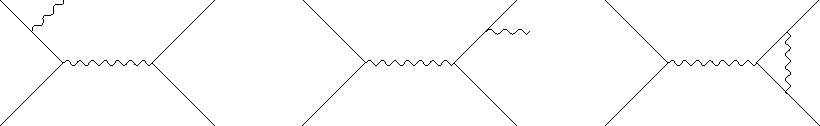
\includegraphics{Images/corr1.pdf}
    \caption*{}
    \labfig{corr1}
\end{figure}\\
These corrections are of order 30\% and are not really interesting, they are basically QED. Then there are corrections coming from QCD which are the same as before with gluons instead of photons but with the difference that gluons can only attach to final state if quarks are present.These QCD corrections only affect the final state.
\begin{figure}[h]
    \centering
    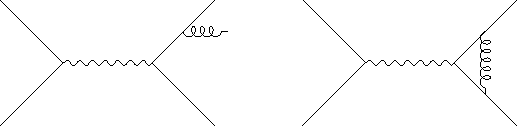
\includegraphics[width=0.7\textwidth]{Images/corr2.pdf}
    \caption*{}
    \labfig{corr2}
\end{figure}\\
\newline
Finally, there are the genuine EW corrections.
\begin{figure}[h]
    \centering
    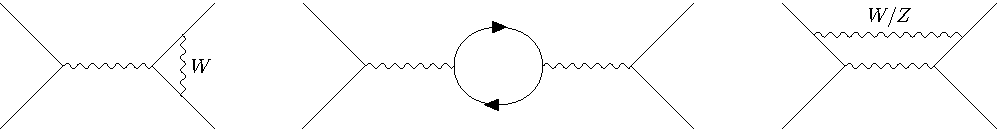
\includegraphics{Images/corr3.pdf}
    \caption*{}
    \labfig{corr3}
\end{figure}\\
These are the ones we are more interested in. It turns out that the contributions from photonic corrections can be removed if we perform the following procedure.
\begin{enumerate}[label=\roman*)]
    \item use an $s$-dependent vacuum polarization, $\alpha_{\text{em}}=\frac{\alpha}{1-\Delta_\alpha(s)}$.
    \item use an $s$-dependent $Z$ width because that also absorbs part of the corrections.
    \[
    \Gamma_Z(s):=\Gamma_Z\left(\frac{s}{m_Z^2}+\varepsilon\frac{s-m_Z^2}{m_Z^2}+\cdots\right)
    \]
    where $\varepsilon$ comes from final state corrections.
    \item define effective couplings which are pseudo-observables.
    \[
    g_{V/A}^f\to(g_{V/A}^f)_{\text{eff}}
    \]
\end{enumerate}
This procedure gives us the possibility of expressing the raw observables, i.e. the ones we measure, with the same form of the tree-level expression. The effective couplings are something that has to be measured, they are parameters that enter in the form of the observables. This is known as the \textbf{Improved Born Approximation} (IBA), it is a way to express observables in a way that mimics the tree-level corrections and subtracts almost entirely the corrections coming from QED and QCD. For example, for the total cross section we get:
\[
\sigma(s)=\frac{12\pi}{m_Z^2}\Gamma_e\Gamma_f\frac{s}{(s-m_Z^2)^2+m_Z^2\Gamma_Z^2(s)}+\sigma_\gamma(s)+\sigma_{\gamma Z}(s)
\]
The decay width $\Gamma_f$ is defined as:
\[
\Gamma_f:=4N_c\Gamma_0\left[(g_V^f)^2_{\text{eff}}R_V^f+(g_A^f)^2_{\text{eff}}R_A^f\right]\sim(g_V^f)_{\text{eff}}^2+(g_A^f)_{\text{eff}}^2 \quad \Gamma_0:=\frac{G_{\text{F}}m_Z^3}{24\sqrt{2}\pi}
\]
$R_V^f$ and $R_A^f$ are numbers that take into account QED and QCD final state radiations. If there were no final state radiations, these two numbers would have been equal to 1. If we measure this quantity, we can then extract $\Gamma_e$ and $\Gamma_f$, i.e. couplings, and also the mass of the $Z$ boson. These coefficients have to be interpreted as pseudo-observables and the other observables can be written in terms of them. In particular, we saw the expression of $A_{\text{FB}}$ in terms of $A_e$ and $A_f$ with the latter given by a tree-level expression which now has to be modified:
\[
A_f:=\frac{2(g_A^f)_{\text{eff}}(g_V^f)_{\text{eff}}}{(g_V^f)_{\text{eff}}^2+(g_A^f)_{\text{eff}}^2}\sim\frac{(g_V^f)_{\text{eff}}/(g_A^f)_{\text{eff}}}{1+[(g_V^f)_{\text{eff}}/(g_A^f)_{\text{eff}}]^2}
\]
The asymmetries depend on the ratio of the couplings while the partial width depends on the sum of the couplings squared. The formulas are the same of the tree-level but now the asymmetries are defined in terms of these pseudo-observables.\\ Other pseudo-observables are the ratio $R_l$ of the hadronic and the leptonic partial width:
\[
R_l:=\frac{\Gamma_h}{\Gamma_l} \quad l=e,\mu,\tau
\]
then there is also $R_{b,c}$ defined as:
\[
R_{b,c}:=\frac{\Gamma_{b,c}}{\Gamma_h}
\]
and the total hadronic cross section:
\[
\sigma_{\text{had}}^0:=12\pi\frac{\Gamma_e\Gamma_h}{m_Z^2\Gamma_Z^2}
\]
Moreover, there is the total invisible width, which is nothing but the $Z$ decay width minus the visible width:
\[
\Gamma_{\text{inv}}:=\Gamma_Z-\Gamma_e-\Gamma_\mu-\Gamma_\tau-\Gamma_{\text{had}}
\]
Another useful redefinition is the one of the effective couplings in terms of other pseudo-observables:
\[
(g_V^f)_{\text{eff}}=\sqrt{\rho_f}(T_3^f-2Q_f\sin^2\theta_{\text{eff}}^f) \quad (g_A^f)_{\text{eff}}=\sqrt{\rho_f}T_3^f
\]
At tree-level, they depend on the quantum numbers of the particle. In order to put everybody on the same page, these couplings have been redefined mimicking the structures of the tree-level expressions. Here two new parameters were introduced, $\rho_f$ and $\sin\theta_{\text{eff}}^f$, with the latter that can be written as:
\[
\sin\theta_{\text{eff}}^f=\frac{1}{|4Q^f|}\left(1-\frac{(g_V^f)_{\text{eff}}^2}{(g_A^f)_{\text{eff}}^2}\right) \quad \text{for}\;T_3^f=\pm\frac{1}{2}
\]
This depends on the ratio between the two effective couplings squared, which means it is a function of the asymmetries that fix this ratio. $\rho_f$ is the corresponding of the $\rho$-parameter we introduced earlier, defined as:
\[
\rho:=\frac{m_W^2}{m_Z^2\cos^2\theta_w}
\]
If there is a virtual exchange of $W$ or $Z$, then the propagator would give a contribution proportional to the inverse squared of the mass of the particle exchanged, $\sim1/m^2_{W/Z}$, times the strength of the coupling. The charged current strength, which is a contact interaction once the heavy states are integrated out, is given by:
\[
G_{\text{F}}^{\text{cc}}\sim\frac{g^2}{m_W^2}
\]
If we do the same for the $Z$, i.e. neutral current, we get:
\[
G_{\text{F}}^{\text{nc}}\sim\frac{g^2}{m_Z^2}+g'^2
\]
The relative importance between charged and neutral current is a ratio of masses and couplings. The $\rho$-parameter then parametrizes the ratio of the strengths of the charged current over the neutral current interaction. For $\rho_f$ is the same story, if it is different from 1 it means that the strength of the charged current is different than neutral current. If it is close to 1, it means there is an effect which is changing this relative importance. These couplings parametrize the 
effective interactions with the $Z$ with respect to the $W$. In other words, instead of defining $\rho_f$ as the ratio of masses, we look at the strength of interactions mediated by the $Z$ and by the $W$.\\
Another observable is $m_W$ if we use the EW scheme where we choose to work with $\alpha_{\text{em}}(0)$ and $G_{\text{F}}$. Again, it is possible to express $m_W$ in terms of a pseudo-observable in the following way:
\[
\left(1-\frac{m_W^2}{m_Z^2}\right)\frac{m_W^2}{m_Z^2}:=\frac{\pi\alpha(m_Z)}{\sqrt{2}G_{\text{F}}m_Z^2(1-\Delta r_w)}
\]
where the new pseudo-observable is $\Delta r_w$. $m_Z$ and $\alpha$ are input parameters, $\alpha$ is computed at $m_Z$ and this effectively incorporates QED corrections in the photon self-energy. Let's check if this formula has a meaning that we are able to understand. At tree-level, $\Delta r_w$ is not present, the ratio of the masses can be written in terms of $g$ and $g'$ and we get:
\[
\underbrace{\left(1-\frac{g^2}{g^2+g'^2}\right)}_{=\frac{g'^2}{g^2+g'^2}=\sin^2\theta_w}\frac{m_W^2}{\cancel{m_Z^2}}=\frac{\pi e^2/4\pi v^2}{\cancel{m_Z^2}}\Rightarrow m_W^2=\frac{v^2}{4}\frac{e^2}{\sin^2\theta_w}=g\frac{v^2}{4} \quad \checkmark\marginnote{$\sqrt{2}G_{\text{F}}=1/v^2$ (we hope)}
\]
At tree-level, everything collapses into things we already know. At one-loop instead, we make an upgrade with this formula to incorporate radiative corrections and we do this by defining a new pseudo-observable in terms of $m_W$. At the end of the day, we have 3 pseudo-observables, $\rho_f, \sin\theta_{\text{eff}}^f$ and $\Delta r_w$. We are now going to define $\Delta\rho_f$ and $\Delta k'^f$ just to reflect the fact that if we switch off the corrections, then $\rho_f=1$ and $\sin\theta_{\text{eff}}^f=\sin\theta_w$.
\[
\left\{
\begin{aligned}
&\rho_f:=1+\Delta\rho_f\\
&\sin\theta_{\text{eff}}^f:=s^2(1+\Delta k'^f)
\end{aligned}
\right.
\quad \text{with}\;s^2:=\frac{1}{2}\left[1-\left(1-\frac{4\pi\alpha(m_Z)}{\sqrt{2}G_{\text{F}}m_Z^2}\right)^{1/2}\right]\xrightarrow[\text{tree-level}]{}\sin^2\theta_w
\]
At this point we have $\{\Delta\rho_f, \Delta k'^f, \Delta r_w\}$, there are three pseudo-observables for each given flavour. We have defined these quantities in such a way that the obvious dependence on the flavour $f$ has been removed, the only dependence on $f$ enters through sub-leading effects like the mass of the quarks in loops or in the final state. The index $f$ will now be dropped because the universality of these parameters is verified. All the information can be condensed in three pseudo-observables if we assume lepton and quarks universality, we now look at the data to see if they support this universality. From LEP collaboration, we get:
\[
\left\{
\begin{aligned}
&R_e=20.804\pm0.050 &&A_{\text{FB}}^e=0.0145\pm0.0025\\
&R_\mu=20.785\pm0.033 &&A_{\text{FB}}^\mu=0.0169\pm0.0013\\
&R_\tau=20.764\pm0.045 &&A_{\text{FB}}^\tau=0.0188\pm0.0017
\end{aligned}
\right.
\]
The data for $R_e, R_\mu$ and $R_\tau$ support universality while for the forward-backward asymmetries there are some differences and one might complain. This difference is coming from the masses and it is an effect which can be parametrized, but we do not want to discuss this so let's pretend universality is true to a very good degree.\\
Another important quantity is the number of neutrinos:
\[
N_\nu:=\frac{\Gamma_{\text{inv}}/\Gamma_l}{(\Gamma_\nu/\Gamma_l)_{\text{SM}}} \quad (N_\nu)_{\text{exp}}=2.9840\pm0.0082
\]
This number should be 3 if everything is according to the SM. Why 3? Because these are the neutrinos in which the $Z$ can decay. Now one might say that in the SM there are no masses for neutrinos, so if we account for these masses maybe there are heavy neutrinos and everything is in agreement. Yes, maybe but we are talking about heavy neutrinos and the $Z$ cannot decay into them. This number is affected only by the light neutrinos, the fact that we get 3 is a test that there are no additional light degrees of freedom to which the $Z$ can decay.\\
The final message is that there is a very good agreement among different experiments, there is evidence of universality and also there is agreement with what we measure in the leptonic sector with what we measure in the quark sector. Everything is pretty consistent, there are some fluctuations but we don't even discuss that. \marginnote[-5cm]{Some references about this topic:\begin{itemize}
    \item \href{https://arxiv.org/abs/hep-ex/0412015}{A Combination of Preliminary Electroweak Measurements and Constraints on the Standard Model}
    \item \href{https://arxiv.org/abs/hep-ex/0509008}{Precision Electroweak Measurements on the Z Resonance}
    \item \href{https://arxiv.org/abs/1012.2367}{Precision Electroweak Measurements and Constraints on the Standard Model}
    \item \href{https://arxiv.org/abs/hep-ph/0402031}{TASI Lectures on Precision Electroweak Physics}
    \item \href{https://arxiv.org/abs/hep-ph/9303304}{Precision Tests of the Standard Model}
    \item \href{https://arxiv.org/abs/hep-ph/9802302}{Precision Physics at LEP}
    \item \href{https://lib-extopc.kek.jp/preprints/PDF/2000/0030/0030731.pdf}{Barbieri Lectures}
\end{itemize}}\\ 
Moving over and going at LEP2, the observables are $e^-e^+\to f\overline{f}$ at different values of $\sqrt{s}$ but there was also the possibility to produce pairs of on-shell $W$ bosons which then can decay in different ways:
\[
e^-e^+\to W^-W^+\to2q2\overline{q}/q\overline{q}l\nu/ll\nu\nu
\]
The first two possibilities are the best ones because it is possible to reconstruct their kinematics. In this way, we can measure the $W$ pole mass and its width,
$\delta m_W\sim30$\,MeV and $\delta\Gamma_W\sim80$\,MeV.\\
The other thing that we can measure in this way are the so-called \textbf{triple gauge couplings} (TGC).
\begin{figure}[h]
    \centering
    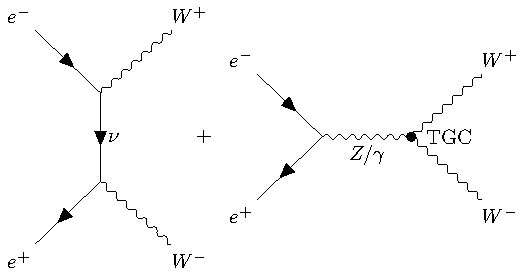
\includegraphics[width=0.7\textwidth]{Images/TGC.pdf}
    \caption*{}
    \labfig{tgc}
\end{figure}\\
This interaction is predicted by the SM, by measuring the cross section of the process we can test the existence of this interaction which was not observed before, it was the first time where a non-abelian interaction between three vector bosons was observed. The first reason to study this process is to study anomalous TGC, the structure of this interaction in the SM is a specific one but there could be other possible interactions in general which can be parametrized in terms of anomalous TGC which we are now going to list. One way to parametrize them is to write all possible local operators which are invariant under U$(1)_{\text{em}}$ and only some of these couplings will be present in the SM while other ones will be anomalous. From the viewpoint of EFT, these couplings come from higher dimensionality operators. Only one interaction comes from dimension 4 operator, which is the kinetic term of the $W$, but then there are higher dimension operators which also involve quartic interactions with possibly more derivative. If we write them in a way that they have to respect U$(1)_{\text{em}}$, we get:
\[
\marginnote{Each operator has a coefficient which is reported between parantheses.}
\left\{
\begin{aligned}
&\gamma_{\mu\nu}W^\mu W^\nu\;\; (k_\gamma) && \gamma_{\nu\nu}W^{\nu\rho}W^\mu_\rho\;\; (\lambda_\gamma)\\
&Z_\mu W^{\mu\nu}W_\nu\;\; (\delta_{g,z}) && Z_{\mu\nu}W^\mu W^\nu\;\; (k_z))\\
&Z_{\mu\nu}W^{\nu\rho}W_\rho^\mu\;\; (\lambda_z)
\end{aligned}
\right.
\]
In the phase where EW symmetry is broken, we have only U$(1)_{\text{em}}$ as a gauge symmetry and we classify all the operators which are invariant under this symmetry which involve three fields. We do it either with one field, which is now not a gauge field anymore it is a spin-1 massless field, or the field strength, defined as $W_{\mu\nu}:=\partial_\mu W_\nu-\partial_\nu W_\mu$.\\
The energy was enough to measure another process, $e^-e^+\to ZZ$, but in this case in the SM there is no possibility these two fields to another vector boson since it should be either a photon or another $Z$ but there are no such interactions in the SM so there is only one diagram.
\begin{figure}[h]
    \centering
    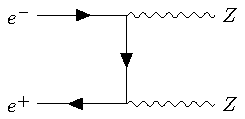
\includegraphics[width=0.45\textwidth]{Images/ZZ.pdf}
    \caption*{}
    \labfig{ZZ}
\end{figure}\\
Again, by measuring the cross section we can test the possible existence of anomalous TGC which can be written as:
\[
\partial_\rho\gamma^{\rho\mu}Z_{\mu\nu}Z^\nu\;\;(f_4^\gamma) \qquad \qquad \partial_\rho Z^{\rho\mu}Z_{\mu\nu}Z^\nu\;\;(f_4^Z)
\]
Beyond LEP and LEP2 there was also Tevatron which played an important role especially in measuring the mass of the $W$ and this is something that is still going on, the later results were published recently. At Tevatron the top quark was discovered, which is important for our EWPT, together with measurements on TGC and $m_W$.
\subsection{Theoretical Calculation}
So far, we discussed the experimental data now we go and discuss the theoretical calculation. First of all, we have to remember that our theory has to be renormalized and instead of using the usual procedure we can do something quicker and use as renormalization parameters three of the observables. Denote now with $a^i_0$ the input observables at tree-level, we then go at one-loop and get some corrections:
\[
a_0^i\xrightarrow[\text{1-loop}]{}a^i=a_0^i+\delta a^i(a_o^i)\xleftrightarrow[\text{invert}]{}a_0^i=a^i-\delta a^i(a_o^i)
\]
Why do we invert such expression? Consider now any observable $S_0$ which is a function of the tree-level input observables:
\[
S_0(a_0^i)\xrightarrow[\text{1-loop}]{}S(a^i)=S_0(a_0^i)+\delta S(a_o^i)=S_0(a^i)-\underbrace{\sum_i\frac{\partial S}{\partial a^i}\delta a^i+\delta S(a^i)}_{\text{full 1-loop corrections}}
\]
The 1-loop corrections are finite, which means the theory is renormalizable: once we have these contributions all divergencies should cancel. Corrections at 1-loop enter in three different ways: corrections to the self-energy, corrections to vertices and then there is everything else to $\mu$-decay except self-energies. Self-energies are written as:
\[
\Pi_{\mu\nu}^{ij}(q)=\eta_{\mu\nu}\left[A^{ij}(0)+q^2F^{ij}(q^2)\right]+\cancel{q_\mu q_\nu\;\text{terms}}
\]
The $q_\mu q_\nu$ terms are negligible, they give a very small contribution proportional to the mass of the electron. The vertices are on-shell, so we are talking about the $Z$-pole and they are parametrized in this way:
\[
-i\frac{e}{s_0c_0}\overline{v}\gamma^\mu(\delta g_V-\gamma_5\delta g_A)u
\]
$s_0$ and $c_0$ are the tree-level expressions for sine and cosine of $\theta_w$, $g_V$ and $g_A$ denote respectively the vector and axial currents. For the corrections to $\mu$-decay they are written as follows:
\[
-i\delta G_{\text{V,B}}[e^-\gamma_\mu(1-\gamma_5)\nu_e][\overline{\nu}_\mu\gamma^\mu(1-\gamma_5)\mu]
\]
All corrections means corrections from box, vertex and fermion self-energy and they are parametrized into the parameter $\delta G_{\text{V,B}}$.\\
The 1-loop corrections are then encoded in $A^{ij}, F^{ij}, \delta g_V, \delta g_A$ and $\delta G_{\text{V,B}}$. Both the input observables $\{\alpha_{\text{em}}(0), G_{\text{F}}, m_Z \}$ and the final output observables will have an expression written in terms of these corrections. $i$ and $j$ can run either on 1,2,3 and $Y$ hypercharge in the SU$(2)\times$U(1) basis or sometimes it is more convenient to rotate to the physical basis where they run on $\pm W,\gamma$ and $Z$. Here we use the physical basis.
\[
\left\{
\begin{aligned}
&\frac{\delta\alpha}{\alpha}=-F^{\gamma\gamma}(0)-2\frac{s}{c}\frac{A^{\gamma Z}(0)}{m_Z^2} &&s^2=1-c^2=\frac{1}{2}\left[1-\left(1-\frac{4\pi\alpha(m_Z^2)}{\sqrt{2}G_{\text{F}}m_Z^2}\right)^{1/2}\right]\\
&\delta m_Z^2=-A^{ZZ}(0)-m_Z^2F^{ZZ}(m_Z^2) &&\frac{\delta G_{\text{F}}}{G_{\text{F}}}=\frac{A^{WW}(0)}{m_W^2}+\frac{\delta G_{\text{V,B}}}{G_{\text{V,B}}}
\end{aligned}
\right.
\]
These are the input observables, then there are the predicted observables which have the following expressions:
\[
\left\{
\begin{aligned}
&m_W^2=m_Z^2c^2+\delta m_W^2-\frac{m_Z^2c^2}{s^2-c^2} \left(s^2\frac{\delta\alpha}{\alpha}-s^2\frac{\delta G_{\text{F}}}{G_{\text{F}}}-c^2\frac{\delta m_Z^2}{m_Z^2}\right)\\
&\Gamma(Z\to l^-l^+)=\frac{G_{\text{F}}m_Z^3}{6\pi\Gamma_Z}\left(1-\frac{\delta G_{\text{F}}}{G_{\text{F}}}-\frac{\delta m_Z^2}{m_Z^2}-F^{ZZ}(m_Z^2)-m_Z^2F'^{ZZ}(m_Z^2)\right)\left[(g_V^0+\Delta g_V)^2+(g_A^0-\Delta g_A)^2\right]\\
&\Delta g_V=-2\frac{s^2c^2}{c^2-s^2}\left(\frac{\delta G_{\text{F}}}{G_{\text{F}}}+\frac{\delta m_Z^2}{m_Z^2}-\frac{\delta\alpha}{\alpha}\right)+\delta g_V+2scF^{\gamma Z}(m_Z^2) \quad \Delta g_A=\delta g_A
\end{aligned}
\right.
\]
where $g_V^0$ and $g_A^0$ denote the tree-level SM couplings. There is also the forward-backward asymmetry, which can be written, assuming lepton universality, as:
\[
A_{\text{FB}}^l=3\frac{(g_V^0+\Delta g_V)^2(g_A^0+\Delta g_A)^2}{\left[(g_V^0+\Delta g_V)^2+(g_A^0+\Delta g_A)^2\right]^2}
\]
That is the same formula as the experimental one but now in terms of theoretical quantities. If we now compare this expression with the formulas of the observables written in terms of the pseudo-observables, we can derive the expression of the pseudo-observables in terms of these theoretical quantities. These are the master formulas, we don't need to compute the pseudo-observables every time. \marginnote{There is a complex system of Chinese boxes but it should be somehow clear.}
\[
\left\{
\begin{aligned}
&\Delta r_w=\frac{\delta G_{\text{F}}}{G_{\text{F}}}+\frac{c^2}{s^2}\frac{\delta m_Z^2}{m_Z^2}-\frac{\delta\alpha}{\alpha}+\frac{s^2-c^2}{c^2}\frac{\delta m_W^2}{m_W^2}\\
&\Delta\rho=-\frac{\delta G_{\text{F}}}{G_{\text{F}}}-\frac{\delta m_Z^2}{m_Z^2}-F^{ZZ}(m_Z^2)-m_Z^2F'^{ZZ}(m_Z^2)-4\Delta g_A\\
&\Delta k=\frac{1}{2s^2}[\Delta g_V-(1-4s^2)\Delta g_A]
\end{aligned}
\right.
\]
All the experimental information can be condensed in these three pseudo-observables and on the theoretical side we just need to compute the quantities arising from 1-loop corrections.\\
How do these theoretical quantities on the mass of the Higgs and on the mass of the top? This was an important question at the time because neither the top nor the Higgs were observed, so this was the only indirect way to get information about their masses. We then want to isolate the observables which are most sensitive to these masses. The mass of the Higgs only enters logarithmically and is in fact very poorly determined, the mass of the top instead enters quadratically so there is a much stronger dependence and now we are going to see why. In particular, these three pseudo-observables depend quadratically on $m_t$ but it turns out that only one linear combination of them depends quadratically on the mass of the top. It is then useful to find a redefinition of the pseudo-observables in terms of other three parameters, the so-called $\varepsilon$ parameters, in such a way that one of them depends quadratically on $m_t$ and the other two do not. That parameter is then the most sensitive to constrain the mass of the top and once the top is discovered is the one most strongly affected. For example, $\Delta\rho$ depends quadratically on $m_t$ and this can be seen as follows. We can rewrite it as:
\[
\Delta\rho=\frac{A^{33}(0)-A^{WW}(0)}{m_W^2}-m_Z^2F'^{ZZ}(m_Z^2)-\frac{\delta G_{\text{V,B}}}{G_{\text{V,B}}}-4\delta g_A
\]
Look now at the first term. It is the self-energy at one loop in which there is either a $W^3W^3$ on the external lines or a $W^+W^-$. These are the loop diagrams of such corrections:
\begin{figure}[h]
    \centering
    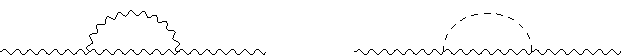
\includegraphics{Images/loopcorr.pdf}
    \caption*{}
    \labfig{loopcorr}
\end{figure}\\
These quantities are convergent despite the fact that each of these contribution is logarithmically divergent. The one on the left goes like $\log(\Lambda/m_Z)$ and the one on the right goes like $\log(\Lambda/m_h)$, where $\Lambda$ is a cut-off. When we go to sum them the contribution is finite, $\sim\log(m_Z/m_h)$.\\
There is a logarithmic dependence on $m_h$ and then there is also the observation that these difference is finite. Is it possible to understand why it is finite and why each of these contributions go like a logarithm? For example, if we do the calculation in the unitary gauge it is not obvious at all, the superficial degree of divergence is larger since there are derivatives in the vertices. It turns out that there is another way to do this calculation which basically rephrases this one in terms of another two-point function which is the one of the would-be Goldstone bosons, which are present in the $\xi$-gauge but not in the unitary one. It is a sort of equivalence theorem, so we look at the kinetic term and its one-loop corrections because when we are in the $\xi$-gauge, the mass term for the vector boson and the kinetic term for the would-be Goldstone boson are packaged in the same term, which looks like this:
\[
|D_\mu\chi^+-m_WW_\mu^+|^2
\]
How can we get this? We write the kinetic term in this way:
\[
\Tr{(D_\mu\Sigma^\dagger)(D^\mu\Sigma)} \quad \Sigma=\exp{i\frac{\chi}{v}}
\]
From one of these two terms we get a derivative and from the other we get the gauge fields by setting $\Sigma$ to the identity. There will be a term which will just be the square of the vector boson field and that is the mass term, but then there is with the same coefficient another term which is the kinetic term for the would-be Goldstone boson. The moral is that if we want to capture this coefficient we can either compute the two-point function of the vector boson or the two-point function of the would-be Goldstone boson in the $\xi$-gauge. In this specific case, this can be done by looking at the following diagrams:
\begin{figure}[h]
    \centering
    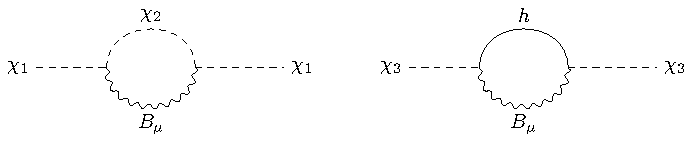
\includegraphics{Images/chi.pdf}
    \caption*{}
    \labfig{chi}
\end{figure}\\
The difference between $A^{33}$ and $A^{WW}$ violates custodial symmetry, in other words it treats $W$ differently from $Z$. $Z$ is written in this strange way, if there was a broken custodial symmetry all components should be equal which means that if we take the difference we should get 0. The non-vanishing of this quantity is a consequence of explicit violation of custodial symmetry. We can get a contribution only if loop diagrams violate custodial symmetry as well. The violation comes because of hypercharge, if we switched it off and took the difference between these two diagrams there would be a perfect cancellation. We then have to exchange $B$ not $W$, because if we exchange something that does not convey the breaking of custodial symmetry we get 0. Remember that we have to look at the kinetic term so let's do power counting: there are two bosonic propagators, there are derivatives in the vertices and this leaves us a logarithmic divergence for both diagrams. If there is a divergence, there should be a counter term: which counter term violates custodial symmetry? There is no such counter term in the SM, the kinetic term for $\chi$ is custodial invariant. Violation of custodial invariance comes from the presence of hypercharge. Therefore, there can be no divergence and the difference must be invariant, and it actually is.\\
Let's now look at the top which is slightly simpler but the argument is basically the same. We go and look at the kinetic term and the contribution from fermions:
\begin{figure}[h]
    \centering
    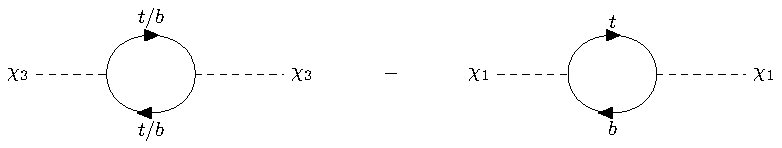
\includegraphics{Images/topbottom.pdf}
    \caption*{}
    \labfig{topbottom}
\end{figure}\\
The vertex comes from the Yukawa coupling:
\[
\overline{q}_L\Sigma\left(\begin{array}{cc}
    t_R & y_t \\
    b_R & y_b
\end{array}\right)
\]
The contribution from the bottom will be small, so we can neglect it and focus on the top. Each diagram will have a logarithmic divergence but the total contribution will be finite and proportional to $y_t^2/16\pi^2$. Here we do not need to gauge anything, this is the gaugeless limit. $y_t^2$ is nothing but $G_{\text{F}}^2m_t^2/16\pi^2$ and the quadratic dependence on the mass of the top is now clear, it comes from the Yukawa interaction not from the gauge one. Altarelli and Barbieri understood that out of these three quantities only one depends quadratically on the mass of the top and they proposed three parameters $\varepsilon_{1,2,3}$ in which only $\varepsilon_1$ depends quadratically on $m_t$ and the other two are combined in a way that there is no such quadratic dependence and they only depend logarithmically on $m_t$.
\[
\varepsilon_1=\Delta\rho \quad \varepsilon_2=c^2\Delta\rho+\frac{s^2}{c^2}\frac{\Delta r_w}{s^2-c^2}-2s^2\Delta k \quad \varepsilon_3=c^2\Delta\rho+(c^2-s^2)\Delta k
\]
We can now write the expression of these parameters in the SM:
\[
\left\{
\begin{aligned}
&\varepsilon_1^{\text{SM}}=\frac{3G_{\text{F}}m_t^2}{8\pi^2\sqrt{2}}-3\frac{G_{\text{F}}m_W^2}{4\pi^2\sqrt{2}}\tan^2\theta_w\log(m_h/m_Z)+\cdots=(5.21\pm0.08)\cdot10^{-3}\\
&\varepsilon_2^{\text{SM}}=-\frac{G_{\text{F}}m_W^2}{2\pi^2\sqrt{2}}\log(m_t/m_Z)+\cdots=-(7.37\pm0.03)\cdot10^{-3}\\
&\varepsilon_3^{\text{SM}}=\frac{G_{\text{F}}m_W^2}{12\pi^2\sqrt{2}}\log(m_h/m_Z)-\frac{G_{\text{F}}m_W^2}{6\pi^2\sqrt{2}}\log(m_t/m_Z)+\cdots=(5.279\pm0.004)\cdot10^{-3}
\end{aligned}
\right.
\]
These are pseudo-observables, not theoretical parameters in such a way that in the SM the dependence on $m_t$ is quadratic only in $\varepsilon_1$. There is in fact a \nth{4} parameter due to the presence of the bottom quark which can be produced in the decay of the $Z$ boson. Moreover, new physics might want to couple preferentially to the bottom, the bottom left in particular, because it is in the same doublet as the top left. There are some models in which the mass of a quark has a relation with the strength of the interaction between the new physics and the SM sector. In other words, if the new physics has to do with EW symmetry breaking then the masses of fermions are coming from EW symmetry breaking, i.e. the larger the mass of a quark the stronger the interaction with the new physics would be. Large mass is possibly a hint of a large interaction and since bottom left is in the same doublet as the top left that means it will also couple strongly to the new sector. This motivates the introduction of an additional parameter $\varepsilon_b$ defined in the following ways:
\[
\rho^b=(1+\Delta\rho)(1+\varepsilon_b)^2 \quad k^b=\frac{1+\Delta k}{1+\varepsilon_b}
\]
Why were two formulas needed to introduce this new parameter and not just one? Because $\varepsilon_b$ parametrizes the shift in the coupling of $b_L$. Remember that we had two couplings, $g_V$ and $g_A$ (or equivalently $g_L$ and $g_R$), written in terms of $\rho$ and $\sin\theta_{\text{eff}}$ which depends on $k$. $\rho$ and $k$ are then functions of $g_L$ and $g_R$, now we want to introduce a non-universal correction only in $g_L$ therefore $\rho$ and $k$ have to be modified in that way. If we move from $V/A$ to $L/R$ only the coupling to bottom left will be modified, the one to bottom right remains untouched. This means that eventually the formula for $\varepsilon_b$ in terms of theoretical parameters which encapsulate one-loop corrections is just:
\[
\varepsilon_b=-2g_{Lb}
\]
In the SM, $\varepsilon_b$ is also proportional to $m_t^2$, which makes it particularly important:
\[
\varepsilon_b^{\text{SM}}=-\frac{G_{\text{F}}m_t^2}{4\pi^2\sqrt{2}}+\cdots=-(6.94\pm0.15)\cdot10^{-3}
\]
How is it possible to understand this quadratic dependence on $m_t$? We go to the gaugeless limit and this dependence is coming from a diagram which has the following form:
\begin{figure}[h]
    \centering
    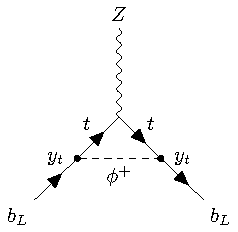
\includegraphics[width=0.45\textwidth]{Images/bl.pdf}
    \caption*{}
    \labfig{bl}
\end{figure}\\
At one-loop, there is the exchange of a $\phi^+$ and if we started with $b_R$ instead the diagram would have been of the same kind but there would have been $y_b$ at the vertices, that is way we do not want to spend another parameter for the corrections to the coupling with $b_R$. To make it simpler, $b_R$ is not in the same multiplet with the top, it is a singlet.\\
Finally, we provide the formulas for the $\varepsilon$ parameters expressed in terms of the theoretical parameters.
\[
\left\{
\begin{aligned}
&\varepsilon_1=e_1-e_5-\frac{\delta G_{\text{V,B}}}{G_{\text{V,B}}}-4\delta g_A &&\varepsilon_3=e_3+c^2e_4-c^2e_5+\frac{c^2-s^2}{2s^2}\delta g_V-\frac{1+2s^2}{2s^2}\delta g_A\\
&\varepsilon_2=e_2-s^2e_4-c^2e_5-\frac{\delta G_{\text{V,B}}}{G_{\text{V,B}}}-\delta g_V-3\delta g_A &&\varepsilon_b=-2\delta g_{Lb}
\end{aligned}
\right.
\]
On the right hand side of these formulas we know everything except for $e_1, e_2, e_3, e_4$ and $e_5$ which are just the self-energies written in this way:
\[
\left\{
\begin{aligned}
&e_1=\frac{A^{33}(0)-A^{WW}(0)}{m_W^2} &&e_2=F^{WW}(m_W^2)-F^{33}(m_Z^2) &&e_3=\frac{c}{s}F^{3B}(m_Z^2)\\
&e_4=F^{\gamma\gamma}(0)-F^{\gamma\gamma}(m_Z^2) &&e_5=m_Z^2F'^{ZZ}(m_Z^2)
\end{aligned}
\right.
\]
These $\varepsilon$ parameters get contribution from all the corrections, not just self-energies. We want to stress again that these $\varepsilon$ parameters parametrize the experimental information in a compact way under the assumption of universality except for the bottom quark, there is no other assumption. This is important because there are also parameters parametrizing the new physics which unfortunately people confuse with these $\varepsilon$ parameters which are pseudo-observables. Fits on the $\varepsilon$ parameters yield the following results, presented also in the plots on the side.\marginnote[-3.5cm]{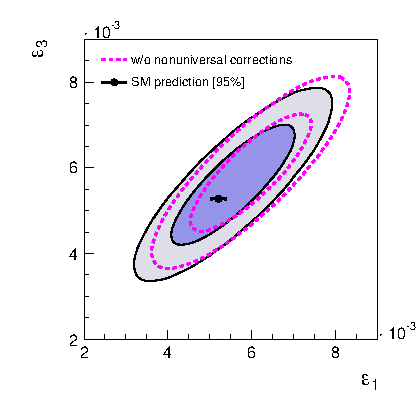
\includegraphics[]{Images/eps1.pdf}
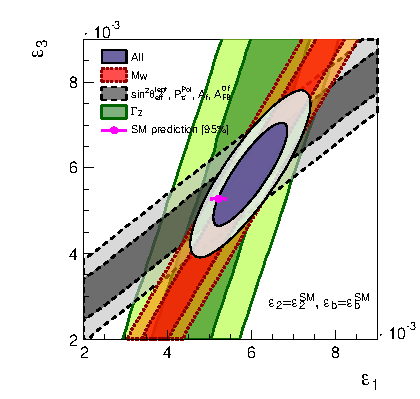
\includegraphics[]{Images/eps2.pdf}\\
Two-dimensional probability distributions for $\varepsilon_1$ and $\varepsilon_3$ in the fit, with floating $\varepsilon_{1,2,3,b}$
(top), or with assuming $\varepsilon_2=\varepsilon_2^{\text{SM}}$ and $\varepsilon_b=\varepsilon_b^{\text{SM}}$ (bottom). In the top plot, the effect of non-universal
vertex corrections is presented. In the bottom plot, we also show the impact of different constraints.
The SM prediction at 95\% is denoted by a point with an error bar. Plots from \cite{Silv}.}
\begin{table}[h]
    \centering
    \begin{tabular}{c|cc}
    \hline
    \rowcolor{gray!45} & Fit $\varepsilon_{1,2,3,b}$ & Fit $\varepsilon_{1,3}$ and $\varepsilon_{2,b}=\varepsilon_{2,b}^{\text{SM}}$\\
    \hline 
    $\varepsilon_1\cdot10^3$ & $5.6\pm1.0$ & $6.0\pm0.6$\\
    $\varepsilon_2\cdot10^3$ & $-7.8\pm0.9$ & $-$\\
    $\varepsilon_3\cdot10^3$ & $5.6\pm0.9$ & $5.9\pm0.8$\\
    $\varepsilon_b\cdot10^3$ & $-5.8\pm1.3$ & $-$\\
    \hline
    \end{tabular}
    \caption*{}
    \labtab{fit}
\end{table}\\
Here there is the assumption of universality but the plots also show effects of non-universal corrections. 
\subsection{Corrections from Heavy New Physics}
How can we improve the fit by including new physics? Remember that $\Gamma$ was proportional to $g_L^2+g_R^2$ while the forward-backward asymmetry $A_{\text{FB}}$ was proportional to $(g_L^2-g_R^2)/(g_L^2+g_R^2)$. For the bottom, the two couplings are equal to:
\[
g_L^b=T_{3L}(b)-Q\sin^2\theta\simeq-0.42 \quad g_R^b=-Q\sin^2\theta\simeq0.077
\]
Apart from the sign, it is clear that $|g_R^b|\ll|g_L^b|$. Hence, we can expand the forward-backward asymmetry as:
\[
A_{\text{FB}}\sim\frac{1-g_R^2/g_L^2}{1+g_R^2/g_L^2}\simeq1-2\frac{g_R^2}{g_L^2}
\]
This means that $g_L$ has to be close to the SM value while we have to find a new model which gives a contribution to the coupling of the bottom right. However, this ratio is small so the model has to give a large correction to $g_R^b$. We then have to find new physics which does not modify $g_L^b$ but gives a large correction to $g_R^b$. The simpler way to get this correction is to get it at tree-level, if we do loops then it becomes smaller. This would be difficult because the model should not destroy other predictions, in particular it does not enter at tree-level $g_L^b$. That is not trivial.\\
We now discuss the corrections coming from new physics in the language of EFTs, i.e. with heavy new physics.\marginnote{Heavy in a sense that it is much heavier than the EW scale.} We are going to do it in a model independent way, considering the SM as an EFT. First of all we are making important assumptions: this new physics is heavy and it gives only oblique corrections, which means that it gives corrections only to vector bosons self-energies. This is not a physical statement, suppose now there is heavy new physics with only higher dimensional operators which affect the self-energies of vector bosons. However, it is always possible to change basis, i.e. make a field redefinition, and rewrite these operators in terms of other operators with the same dimensionality. If the corrections are oblique in one basis they will not be oblique in another basis so the statement is that we are assuming there exists some basis in which the corrections are only to the self-energies, that is the physical statement. Self-energies are parametrized as $\Pi_{\mu\nu}^{ij}(q)$ where $q$ is the incoming momentum, there will be several of these quantities and what we can do is write a sort of effective Lagrangian quadratic in the gauge fields in which we write all possible terms whose coefficients are $\Pi_{\mu\nu}$. Let's say that the scale of new physics is such that $\Lambda_{\text{NP}}\gg m_{W,Z,h}$, $\Pi_{\mu\nu}$ can always be expanded in powers of $q^2/\Lambda_{\text{NP}}^2$ and if we truncate the expansion we are left with an effective Lagrangian. Working in the base where EW symmetry is broken but electromagnetism is preserved, we have:
\[
\pazocal{L}_{\text{eff}}=W_\mu^+\Pi_{WW}^{\mu\nu}(q)W_\nu^-+W_\mu^3\Pi_{33}^{\mu\nu}W_\nu^3+B_\mu\Pi_{BB}^{\mu\nu}B_\nu+W_\mu^3\Pi_{3B}^{\mu\nu}B_\nu+\cdots
\]
where $\cdots$ represents terms higher in the number of fields. This is the most general effective Lagrangian we can write, invariant under electromagnetism and quadratic in the fields. How do these form factors look like? They can be written as:
\[
\Pi_{\mu\nu}^{ij}(q)=\eta_{\mu\nu}\Pi^{ij}(q^2)+\cancel{q_\mu q_\nu\;\text{terms}} \quad \Pi^{ij}(q^2)=A^{ij}(0)+q^2F^{ij}(q^2)
\]
The $q_\mu q_\nu$ terms can be neglected, so our form factors are just scalar functions of $q^2$. If the new physics is heavy, then we can think of expanding these form factors in powers of $q^2/\Lambda_{\text{NP}}^2$ and there will be some SM contributions but now we just want to focus on the new physics contribution. 
\[
\Pi(q^2)=\Pi(0)+q^2\Pi'(q^2)+\frac{(q^2)^2}{2}\Pi''(q^2)+\cdots
\]
Where should we stop in this expansion? Consider now the first piece in $\pazocal{L}_{\text{eff}}$: there are $\Pi_{WW}(0)$ and $\Pi_{WW}'(0)$.\marginnote{We will use a non-standard normalization of fields, in particular they will be normalized with the couplings in front of the kinetic terms: $-F_{\mu\nu}^2/4g^2$.} These quantities have to reproduce the $W$ mass, so if we look at 0 momentum we have:
\[
\Pi_{WW}(0)=\frac{v^2}{4} \quad \Pi_{WW}'(0)=\frac{1}{g^2}
\]
Similarly, $\Pi'_{BB}(0)=1/g'^2$ and we are not able to test new physics with these parameters. The other quantities we can consider are the remaining three form factors at 0 momentum which form a matrix:
\[
\left(\begin{array}{cc}
    \Pi_{33}(0) & \Pi_{3B}(0) \\
    \Pi_{3B}(0) & \Pi_{BB}(0) 
\end{array}\right)
\]
This matrix has to satisfy some requirements:
\begin{enumerate}[label=\roman*)]
    \item there should be 0 as eigenvalue because these are the masses of the photon and the $Z$. This means that we are requiring that the photon must be massless:
    \[
    \Pi_{33}(0)\Pi_{BB}(0)-\Pi_{3B}^2(0)=0
    \]
    \item Photon must couple to the usual charge generator $Q=T_3+Y$
\end{enumerate}
This means in practice that this matrix has to be proportional to the following:\marginnote{In the standard normalization it will be:
\[
\left(\begin{array}{cc}
    g^2 & gg' \\
    gg' & g'^2 
\end{array}\right)
\]
but now we are in the non-standard normalization so the couplings are removed.}
\[
\left(\begin{array}{cc}
    \Pi_{33}(0) & \Pi_{3B}(0) \\
    \Pi_{3B}(0) & \Pi_{BB}(0) 
\end{array}\right)\propto\left(\begin{array}{cc}
    1 & 1 \\
    1 & 1 
\end{array}\right)
\]
There will then be constraints on these parameters:
\[
\Pi_{33}(0)=\Pi_{BB}(0)=\Pi_{3B}(0)
\]
2 conditions for 3 quantities. If we truncated the series at second derivative, we would have $4\cdot3=12$ parameters, minus the 5 conditions leaves us with 7 parameters. These are the ones which parametrize the new physics, the others will receive contributions from them. Do we have to keep all of them? The idea is that there should be a hierarchy, some parameters will be smaller than the other ones so why would we want to keep them? Because some of the $\Pi'$ are already fixed, so if we want to consider corrections from new physics for such quantities we have to go to the second order which represents the first correction. It is not a matter of truncating the expansion a-priori, we have to see for each parameter what is the first leading order correction coming from new physics and that is when we stop. This first correction does not appear at the same level in all the channels. 
\begin{table}[h]
    \centering
    \begin{tabular}{c|cc}
    \hline
    \rowcolor{gray!45} Does it break: &SU$(2)_{\text{EW}}$ & Custodial symmetry \\
    \hline 
    $\Pi'_{3B}(0),\cancel{\Pi''_{3B}(0)}$ & \checkmark & \xmark\\
    $\Pi_{33}(0)-\Pi_{WW}(0)$ & \checkmark & $\checkmark$\\
    $\cancel{\Pi'_{33}(0)-\Pi'_{WW}(0)}$ & \checkmark & $\checkmark$\\
    $\cancel{\Pi''_{33}(0)-\Pi''_{WW}(0)}$ & \checkmark & \checkmark\\
    $\Pi_{BB}''(0)$ & \xmark & \xmark\\
    $\Pi_{WW}''(0)$ & \xmark & \xmark\\
    \hline
    \end{tabular}
    \caption*{}
    \labtab{boh}
\end{table}\\
These are the 7 parameters written in this linear combination. Notice that some of them have been crossed out because they are not useful: $\Pi''_{3B}(0)$ can be ignored because if new physics contribute to $\Pi'_{3B}(0)$ then it will contribute to $\Pi''_{3B}(0)$ in a suppressed way. The same story applies for $[\Pi'_{33}(0)-\Pi'_{WW}(0)]$ and $[\Pi''_{33}(0)-\Pi''_{WW}(0)]$. We are then left with 4 parameters encoding the oblique  effects of new physics. These parameters have a name:
\[
\left\{
\begin{aligned}
&\hat{T}:=\frac{g^2}{m_W^2}\left\{[\Pi_{33}(0)-\Pi_{WW}(0)]-[\Pi_{33}^{\text{SM}}(0)-\Pi_{WW}^{\text{SM}}(0)]\right\}\\
&\hat{S}:=g^2[\Pi_{33}'(0)-\Pi_{33}'^{\text{SM}}(0)]\\
&\hat{W}:=\frac{g^2m_W^2}{2}[\Pi_{WW}''0)-\Pi_{WW}''^{\text{SM}}(0)]\\
&\hat{Y}:=\frac{g'^2m_W^2}{2}[\Pi_{BB}''^{\text{SM}}(0)-\Pi_{BB}''^{\text{SM}}(0)]
\end{aligned}
\right.
\]
The subtraction of the SM quantities are due to the fact that we want to keep only the new physics contribution. It is now possible to connect these quantities with the $\varepsilon$ parameters.
\[
\varepsilon_i=\varepsilon_i^{\text{SM}}+\varepsilon_i^{\text{NP}}\quad \Delta\varepsilon_i^{\text{NP}}=\Delta\varepsilon_i^{\text{SD}}+\Delta\varepsilon_i^{\text{LD}}
\]
The new physics contribution can be splitted in a term deriving from short distance (SD) and a term from long distance (LD). If we have diagrams in which only heavy particles circulate in the loops then we can see this effect as a point-like interaction, i.e. a local operator. That is the short distance but it could be that new physics modifies properties of the SM particles, in particular their couplings, and then there would be new physics effects in diagrams where there are SM particles circulating in the loop with modified couplings. This is long distance.\\
The short distance contribution is parametrized in terms of the parameters $\hat{T}, \hat{S}, \hat{W}$ and $\hat{Y}$.
\[
\left\{
\begin{aligned}
&\Delta\varepsilon_1^{\text{SD}}=\hat{T}-\hat{W}-\frac{s^2}{c^2}\hat{Y} &&\Delta\varepsilon_2^{\text{SD}}=-\hat{W}\\
&\Delta\varepsilon_3^{\text{SD}}=\hat{S}-\hat{W}-\hat{Y} &&\Delta\varepsilon_b^{\text{SD}}=0
\end{aligned}
\right.
\]
There is another approach done in the '90s by Peskin and Takeuchi.\marginnote{Some references: \href{https://journals.aps.org/prl/abstract/10.1103/PhysRevLett.65.964}{New constraint on a strongly interacting Higgs sector} and \href{https://journals.aps.org/prd/abstract/10.1103/PhysRevD.46.381}{Estimation of oblique electroweak corrections}} They did something very similar but they made a conceptual mistake because they thought of truncating the expansion at first order independently on the channel they were looking at. Basically they were neglecting $\hat{W}$ and $\hat{Y}$, since they appear at second order derivatives, but they were including one more.
\[
\left\{
\begin{aligned}
&\hat{S}:=16\pi[\Pi'_{33}(0)-\Pi_{33}'^{\text{SM}}(0)]\\
&\hat{T}:=\frac{4\pi}{s^2c^2m_Z^2}\left\{[\Pi_{11}(0)-\Pi_{33}(0)]-[\Pi_{11}^{\text{SM}}(0)-\Pi_{33}^{\text{SM}}(0)]\right\}\\
&\hat{U}:=16\pi\left\{[\Pi'_{WW}(0)-\Pi'_{33}(0)]-[\Pi_{11}'^{\text{SM}}(0)-\Pi_{11}'^{\text{SM}}(0)]\right\}
\end{aligned}
\right.
\]
There are 3 parameters now instead of 4 but there is a problem because this basis is neither complete nor minimal, the $\hat{U}$ parameter is useless because if new physics contributes to $\hat{U}$ it will also contribute to $\hat{T}$, which is the leading effect. If new physics instead is not heavy we should not do this and look at the $\varepsilon$ parameters because they are capturing everything. The $\varepsilon$ parameters are pseudo-observables, they have nothing to do with theoretical calculations, they are not assuming that the new physics is heavy while here $\hat{S}, \hat{T}$ and $\hat{U}$ are parametrizing heavy new physics.\\
We now want to show what are the dimension 6 operators which correspond to these parameters:
\[
\left\{
\begin{aligned}
&\hat{T}:\; O_T=(H^\dagger\overset{\leftrightarrow}{D_\mu}H)^2 \quad \hat{W}:\;O_{WW}=(D_\mu W^{\mu\nu,a})^2 \quad \hat{Y}:\; O_{BB}=(\partial_\mu B^{\mu\nu})^2\\
&\hat{S}:\;O_W=H^\dagger T^a\overset{\leftrightarrow}{D_\mu}HD_\nu W^{\mu\nu,a} \quad O_B=H^\dagger\overset{\leftrightarrow}{D_\mu}H\partial_\nu B^{\mu\nu}\to\hat{S}\approx O_W-O_B
\end{aligned}
\right.
\]
\marginnote[-1cm]{There is also another basis in which we can introduce the operator: 
\[
O_{WB}:=H^\dagger T^aW_{\mu\nu}^aB^{\mu\nu}H
\]
}
There are 4 parameters however under the assumption of universality there are only 3 $\varepsilon$ parameters, 3 pseudo-observables. Hence, it is not possible to use only LEP1 data to extract values of all these 4 parameters and we have to go to LEP2 which is measuring also the cross section of $e^-e^+\to f\overline{f}$ at different values of the energy and that gives other experimental inputs to fit the 4 parameters. It turns out that $\hat{W}$ and $\hat{Y}$ are like, within the precision we have, contact interaction among 4 fermions. We are doing this type of scattering:
\begin{figure}[h]
    \centering
    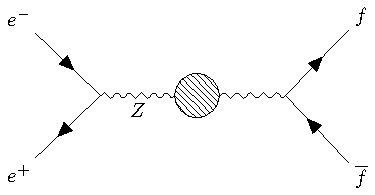
\includegraphics[width=0.6\textwidth]{Images/4fblob.pdf}
    \caption*{}
    \labfig{4fblob}
\end{figure}\\
The propagator in this diagram is given by:
\[
\frac{i}{q^2-m_Z^2+\frac{q^4\hat{W}}{m_Z^2}}
\]
The new physics effects correct this self-energy at order $q^4$. We are at LEP, so we can pretend that $q^2\approx(200\,\text{GeV})^2\gg m_Z^2\simeq(90\,\text{GeV})^2$ and the corrections associated to $\hat{W}$ have to be much smaller than $q^2$ because we are assuming it is a small effect with respect to the SM contribution. It turns out that $\hat{W}$ is constrained to the level of $10^{-3}$ so it is a good approximation, everything is consistent. We can then expand this propagator:
\begin{align*}
\frac{i}{q^2-m_Z^2+\frac{q^4\hat{W}}{m_Z^2}}&\simeq\frac{i}{q^2-m_Z^2}\left(1-\frac{q^4\hat{W}}{m_Z^2}\frac{i}{q^2-m_Z^2}\right)[1+\pazocal{O}(\hat{W})]\underset{\mathclap{\tikz \node {$\uparrow$} node [below=1ex] {\footnotesize $q^2\gg m_Z^2$ };}}{\simeq}\frac{i}{q^2-m_Z^2}\left(1-\frac{q^2}{m_Z^2}\hat{W}\right)[1+\pazocal{O}(\hat{W})]\\
&\simeq\frac{i}{q^2-m_Z^2}-\frac{\hat{W}}{m_Z^2}+\pazocal{O}(\hat{W}/q^2)
\end{align*}
Notice that now the second term does not depend on $q^2$ and it is a contact interaction, we can see it diagrammatically as:
\begin{figure}[h]
    \centering
    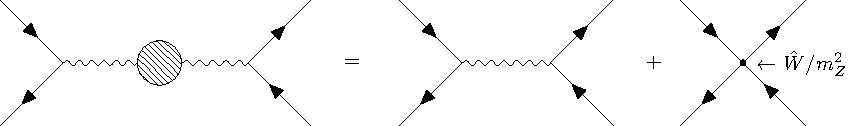
\includegraphics{Images/contact.pdf}
    \caption*{}
    \labfig{contact}
\end{figure}\\
It is also possible to obtain the same result by doing a field redefinition and rewrite $O_{WW}$ in terms of a four-fermion operator which is still dimension 6. That is true, it is possible to exhibit such a field redefinition.\\
We have seen that the $\Delta\varepsilon_i$ contribution to new physics came from two pieces, a short distance term and a long distance one. We computed the short distance term in the framework of EFT by saying that at tree-level there is one operator which contributes to each parameter. However, there was a simplification in this story because what we have said is true but who is stopping us from going at loop-level? We should also worry about the short distance contribution coming by making loops with insertions with higher dimension operators. For example, if we want to get a contribution to $\hat{T}$ we look at:
\begin{figure}[h]
    \centering
    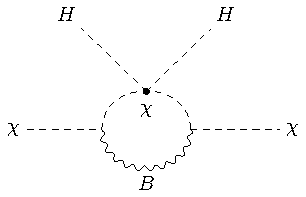
\includegraphics[width=0.45\textwidth]{Images/t.pdf}
    \caption*{}
    \labfig{t}
\end{figure}\\
The higher dimension operator which have been inserted in the vertex above is $O_H:=(\partial_\mu H^\dagger H)^2$ and we get a correction to $\hat{T}$. However, if we make such a diagram we obtain a logarithmic divergence since there is one derivative in each of the remaining vertices. This diagram will then go like:
\[
\frac{1}{\epsilon}\log(\mu/m_Z)\frac{g'^2}{16\pi^2}C_H=\Delta C_T
\]
This means that we need a counter term to cancel this divergence, such counter term will be of the following form:
\begin{figure}[h]
    \centering
    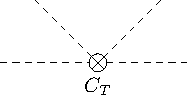
\includegraphics[width=0.35\textwidth]{Images/ct.pdf}
    \caption*{}
    \labfig{ct}
\end{figure}\\
The counter term is $O_T$ itself so it appears by considering $C_T$ as a function of $\mu$, exactly like in QED. There is a simple argument using dimensional analysis which tells us that if in our theory there is no relevant operator\marginnote{Relevant means dimensionality smaller than 4.} then there are only dimensionless couplings in the Lagrangian at dimension 4. If we do a diagram where we insert a dimension 6 operator, there is a parameter which has dimension $-2$ and if this diagram gives a logarithmic divergence the counter term cancelling such divergence will necessarily be a dimension 6 operator. Of course if we do more than one insertion things change, e.g. for two insertions the dimension will be 8 and the effects will be suppressed. Making diagrams with one insertion of a dimension 6 operator is a normalization of other dimension 6 operators. When we do loops, we will be able to pull out powers of the mass, e.g. mass of the Higgs, and that term would somehow help us balance the presence of this coefficient. This in fact increases the degree of divergence at least in principle but since we are using dimensional regularization eventually everything will be inside the logarithmic divergence, which in this case would be proportional to $m_h^2C_H^2$ and that corresponds to a renormalization of $(H^\dagger H)^2$.\\
The moral is that $C_T(\mu)$ is given by:
\[
C_T(\mu)=C_T(\Lambda)+\frac{g'^2}{16\pi^2}\log(\Lambda/\mu)C_H(\Lambda)
\]
We discovered that at tree-level $\varepsilon_1$ gets a contribution from $C_T$ but now we see that $C_T$ depends on $\mu$ so which scale should we use? There are effects which come from loops of SM particles but this effect is short distance because it comes from a divergence. The divergence is coming from high energies so we can use a formalism which is SU(2) invariant, we are not sensitive to the breaking of SU(2). We are looking at diagrams in which we use SU(2) quantum numbers, there is no need to go to the broken phase and because there are loops of light particles but with a divergent contribution, this divergent contribution is always coming from internal momenta. We can incorporate this in the short distance contribution and at this point $\hat{T}$ will be proportional to $C_T$ at some low scale, e.g. $m_Z$. We then incorporate the scale at which we match the full theory with the EFT, that is the scale at which the new particles will appear, and then we run the effective operators to the scale at which we do the experiment, in this case $m_Z$, and there will be a short distance contribution which we can incorporate by resolving the RGE equation.\\
If we use a different scale, e.g. $m_W$ or $m_h$, this would differ by something which is finite and that contribution can always be incorporated into the long distance part which is still present. The way in which this short distance contribution is defined is a bit ambiguous but the ambiguity can be reabsorbed in the long distance contribution.  
\end{document}
